\documentclass[twoside]{book}

% Packages required by doxygen
\usepackage{fixltx2e}
\usepackage{calc}
\usepackage{doxygen}
\usepackage{graphicx}
\usepackage[utf8]{inputenc}
\usepackage{makeidx}
\usepackage{multicol}
\usepackage{multirow}
\PassOptionsToPackage{warn}{textcomp}
\usepackage{textcomp}
\usepackage[nointegrals]{wasysym}
\usepackage[table]{xcolor}

% Font selection
\usepackage[T1]{fontenc}
\usepackage{mathptmx}
\usepackage[scaled=.90]{helvet}
\usepackage{courier}
\usepackage{amssymb}
\usepackage{sectsty}
\renewcommand{\familydefault}{\sfdefault}
\allsectionsfont{%
  \fontseries{bc}\selectfont%
  \color{darkgray}%
}
\renewcommand{\DoxyLabelFont}{%
  \fontseries{bc}\selectfont%
  \color{darkgray}%
}
\newcommand{\+}{\discretionary{\mbox{\scriptsize$\hookleftarrow$}}{}{}}

% Page & text layout
\usepackage{geometry}
\geometry{%
  a4paper,%
  top=2.5cm,%
  bottom=2.5cm,%
  left=2.5cm,%
  right=2.5cm%
}
\tolerance=750
\hfuzz=15pt
\hbadness=750
\setlength{\emergencystretch}{15pt}
\setlength{\parindent}{0cm}
\setlength{\parskip}{0.2cm}
\makeatletter
\renewcommand{\paragraph}{%
  \@startsection{paragraph}{4}{0ex}{-1.0ex}{1.0ex}{%
    \normalfont\normalsize\bfseries\SS@parafont%
  }%
}
\renewcommand{\subparagraph}{%
  \@startsection{subparagraph}{5}{0ex}{-1.0ex}{1.0ex}{%
    \normalfont\normalsize\bfseries\SS@subparafont%
  }%
}
\makeatother

% Headers & footers
\usepackage{fancyhdr}
\pagestyle{fancyplain}
\fancyhead[LE]{\fancyplain{}{\bfseries\thepage}}
\fancyhead[CE]{\fancyplain{}{}}
\fancyhead[RE]{\fancyplain{}{\bfseries\leftmark}}
\fancyhead[LO]{\fancyplain{}{\bfseries\rightmark}}
\fancyhead[CO]{\fancyplain{}{}}
\fancyhead[RO]{\fancyplain{}{\bfseries\thepage}}
\fancyfoot[LE]{\fancyplain{}{}}
\fancyfoot[CE]{\fancyplain{}{}}
\fancyfoot[RE]{\fancyplain{}{\bfseries\scriptsize Generated on Thu Sep 18 2014 05\+:51\+:59 for Chess\+Project by Doxygen }}
\fancyfoot[LO]{\fancyplain{}{\bfseries\scriptsize Generated on Thu Sep 18 2014 05\+:51\+:59 for Chess\+Project by Doxygen }}
\fancyfoot[CO]{\fancyplain{}{}}
\fancyfoot[RO]{\fancyplain{}{}}
\renewcommand{\footrulewidth}{0.4pt}
\renewcommand{\chaptermark}[1]{%
  \markboth{#1}{}%
}
\renewcommand{\sectionmark}[1]{%
  \markright{\thesection\ #1}%
}

% Indices & bibliography
\usepackage{natbib}
\usepackage[titles]{tocloft}
\setcounter{tocdepth}{3}
\setcounter{secnumdepth}{5}
\makeindex

% Custom commands
\newcommand{\clearemptydoublepage}{%
  \newpage{\pagestyle{empty}\cleardoublepage}%
}


%===== C O N T E N T S =====

\begin{document}

% Titlepage & ToC
\pagenumbering{roman}
\begin{titlepage}
\vspace*{7cm}
\begin{center}%
{\Large Chess\+Project }\\
\vspace*{1cm}
{\large Generated by Doxygen 1.8.8}\\
\vspace*{0.5cm}
{\small Thu Sep 18 2014 05:51:59}\\
\end{center}
\end{titlepage}
\clearemptydoublepage
\tableofcontents
\clearemptydoublepage
\pagenumbering{arabic}

%--- Begin generated contents ---
\chapter{Namespace Index}
\section{Packages}
Here are the packages with brief descriptions (if available)\+:\begin{DoxyCompactList}
\item\contentsline{section}{{\bf chess} }{\pageref{namespacechess}}{}
\item\contentsline{section}{{\bf chess.\+base\+Objects} }{\pageref{namespacechess_1_1base_objects}}{}
\item\contentsline{section}{{\bf chess.\+custom} }{\pageref{namespacechess_1_1custom}}{}
\item\contentsline{section}{{\bf chess.\+gamemodes} }{\pageref{namespacechess_1_1gamemodes}}{}
\item\contentsline{section}{{\bf chess.\+general} }{\pageref{namespacechess_1_1general}}{}
\item\contentsline{section}{{\bf chess.\+gui} }{\pageref{namespacechess_1_1gui}}{}
\item\contentsline{section}{{\bf chess.\+master} }{\pageref{namespacechess_1_1master}}{}
\item\contentsline{section}{{\bf chess.\+pieces} }{\pageref{namespacechess_1_1pieces}}{}
\end{DoxyCompactList}

\chapter{Hierarchical Index}
\section{Class Hierarchy}
This inheritance list is sorted roughly, but not completely, alphabetically\+:\begin{DoxyCompactList}
\item \contentsline{section}{chess.\+base\+Objects.\+Board}{\pageref{classchess_1_1base_objects_1_1_board}}{}
\item \contentsline{section}{chess.\+base\+Objects.\+Event}{\pageref{classchess_1_1base_objects_1_1_event}}{}
\item \contentsline{section}{chess.\+custom.\+Faction}{\pageref{enumchess_1_1custom_1_1_faction}}{}
\item \contentsline{section}{chess.\+base\+Objects.\+Game}{\pageref{classchess_1_1base_objects_1_1_game}}{}
\item \contentsline{section}{chess.\+base\+Objects.\+Game\+Mode}{\pageref{classchess_1_1base_objects_1_1_game_mode}}{}
\begin{DoxyCompactList}
\item \contentsline{section}{chess.\+gamemodes.\+Classic\+Chess}{\pageref{classchess_1_1gamemodes_1_1_classic_chess}}{}
\end{DoxyCompactList}
\item \contentsline{section}{chess.\+base\+Objects.\+History}{\pageref{classchess_1_1base_objects_1_1_history}}{}
\item J\+Panel\begin{DoxyCompactList}
\item \contentsline{section}{chess.\+base\+Objects.\+Drawable\+Object}{\pageref{classchess_1_1base_objects_1_1_drawable_object}}{}
\begin{DoxyCompactList}
\item \contentsline{section}{chess.\+base\+Objects.\+Piece}{\pageref{classchess_1_1base_objects_1_1_piece}}{}
\begin{DoxyCompactList}
\item \contentsline{section}{chess.\+pieces.\+Bishop}{\pageref{classchess_1_1pieces_1_1_bishop}}{}
\item \contentsline{section}{chess.\+pieces.\+King}{\pageref{classchess_1_1pieces_1_1_king}}{}
\item \contentsline{section}{chess.\+pieces.\+Knight}{\pageref{classchess_1_1pieces_1_1_knight}}{}
\item \contentsline{section}{chess.\+pieces.\+Pawn}{\pageref{classchess_1_1pieces_1_1_pawn}}{}
\item \contentsline{section}{chess.\+pieces.\+Queen}{\pageref{classchess_1_1pieces_1_1_queen}}{}
\item \contentsline{section}{chess.\+pieces.\+Rook}{\pageref{classchess_1_1pieces_1_1_rook}}{}
\end{DoxyCompactList}
\item \contentsline{section}{chess.\+base\+Objects.\+Square}{\pageref{classchess_1_1base_objects_1_1_square}}{}
\end{DoxyCompactList}
\end{DoxyCompactList}
\item \contentsline{section}{chess.\+gui.\+Main\+Menu}{\pageref{classchess_1_1gui_1_1_main_menu}}{}
\item \contentsline{section}{chess.\+base\+Objects.\+Move\+Style}{\pageref{classchess_1_1base_objects_1_1_move_style}}{}
\item \contentsline{section}{chess.\+gui.\+New\+Game\+Menu}{\pageref{classchess_1_1gui_1_1_new_game_menu}}{}
\item \contentsline{section}{chess.\+base\+Objects.\+Player}{\pageref{classchess_1_1base_objects_1_1_player}}{}
\item \contentsline{section}{chess.\+master.\+Runner}{\pageref{classchess_1_1master_1_1_runner}}{}
\item \contentsline{section}{chess.\+base\+Objects.\+Team}{\pageref{classchess_1_1base_objects_1_1_team}}{}
\item \contentsline{section}{chess.\+base\+Objects.\+Turn}{\pageref{classchess_1_1base_objects_1_1_turn}}{}
\item \contentsline{section}{chess.\+general.\+Utilities}{\pageref{classchess_1_1general_1_1_utilities}}{}
\item Action\+Listener\begin{DoxyCompactList}
\item \contentsline{section}{chess.\+gui.\+Main\+Menu.\+Load\+Game\+Listener}{\pageref{classchess_1_1gui_1_1_main_menu_1_1_load_game_listener}}{}
\item \contentsline{section}{chess.\+gui.\+Main\+Menu.\+New\+Game\+Listener}{\pageref{classchess_1_1gui_1_1_main_menu_1_1_new_game_listener}}{}
\item \contentsline{section}{chess.\+gui.\+Main\+Menu.\+Quit\+Listener}{\pageref{classchess_1_1gui_1_1_main_menu_1_1_quit_listener}}{}
\item \contentsline{section}{chess.\+gui.\+Main\+Menu.\+Settings\+Listener}{\pageref{classchess_1_1gui_1_1_main_menu_1_1_settings_listener}}{}
\end{DoxyCompactList}
\item Default\+Table\+Cell\+Renderer\begin{DoxyCompactList}
\item \contentsline{section}{chess.\+base\+Objects.\+Board.\+Chess\+Board\+Cell\+Renderer}{\pageref{classchess_1_1base_objects_1_1_board_1_1_chess_board_cell_renderer}}{}
\end{DoxyCompactList}
\end{DoxyCompactList}

\chapter{Class Index}
\section{Class List}
Here are the classes, structs, unions and interfaces with brief descriptions\+:\begin{DoxyCompactList}
\item\contentsline{section}{{\bf chess.\+pieces.\+Bishop} }{\pageref{classchess_1_1pieces_1_1_bishop}}{}
\item\contentsline{section}{{\bf chess.\+base\+Objects.\+Board} }{\pageref{classchess_1_1base_objects_1_1_board}}{}
\item\contentsline{section}{{\bf chess.\+base\+Objects.\+Board.\+Chess\+Board\+Cell\+Renderer} }{\pageref{classchess_1_1base_objects_1_1_board_1_1_chess_board_cell_renderer}}{}
\item\contentsline{section}{{\bf chess.\+gamemodes.\+Classic\+Chess} }{\pageref{classchess_1_1gamemodes_1_1_classic_chess}}{}
\item\contentsline{section}{{\bf chess.\+base\+Objects.\+Drawable\+Object} }{\pageref{classchess_1_1base_objects_1_1_drawable_object}}{}
\item\contentsline{section}{{\bf chess.\+base\+Objects.\+Event} }{\pageref{classchess_1_1base_objects_1_1_event}}{}
\item\contentsline{section}{{\bf chess.\+custom.\+Faction} }{\pageref{enumchess_1_1custom_1_1_faction}}{}
\item\contentsline{section}{{\bf chess.\+base\+Objects.\+Game} }{\pageref{classchess_1_1base_objects_1_1_game}}{}
\item\contentsline{section}{{\bf chess.\+base\+Objects.\+Game\+Mode} }{\pageref{classchess_1_1base_objects_1_1_game_mode}}{}
\item\contentsline{section}{{\bf chess.\+base\+Objects.\+History} }{\pageref{classchess_1_1base_objects_1_1_history}}{}
\item\contentsline{section}{{\bf chess.\+pieces.\+King} }{\pageref{classchess_1_1pieces_1_1_king}}{}
\item\contentsline{section}{{\bf chess.\+pieces.\+Knight} }{\pageref{classchess_1_1pieces_1_1_knight}}{}
\item\contentsline{section}{{\bf chess.\+gui.\+Main\+Menu.\+Load\+Game\+Listener} }{\pageref{classchess_1_1gui_1_1_main_menu_1_1_load_game_listener}}{}
\item\contentsline{section}{{\bf chess.\+gui.\+Main\+Menu} }{\pageref{classchess_1_1gui_1_1_main_menu}}{}
\item\contentsline{section}{{\bf chess.\+base\+Objects.\+Move\+Style} }{\pageref{classchess_1_1base_objects_1_1_move_style}}{}
\item\contentsline{section}{{\bf chess.\+gui.\+Main\+Menu.\+New\+Game\+Listener} }{\pageref{classchess_1_1gui_1_1_main_menu_1_1_new_game_listener}}{}
\item\contentsline{section}{{\bf chess.\+gui.\+New\+Game\+Menu} }{\pageref{classchess_1_1gui_1_1_new_game_menu}}{}
\item\contentsline{section}{{\bf chess.\+pieces.\+Pawn} }{\pageref{classchess_1_1pieces_1_1_pawn}}{}
\item\contentsline{section}{{\bf chess.\+base\+Objects.\+Piece} }{\pageref{classchess_1_1base_objects_1_1_piece}}{}
\item\contentsline{section}{{\bf chess.\+base\+Objects.\+Player} }{\pageref{classchess_1_1base_objects_1_1_player}}{}
\item\contentsline{section}{{\bf chess.\+pieces.\+Queen} }{\pageref{classchess_1_1pieces_1_1_queen}}{}
\item\contentsline{section}{{\bf chess.\+gui.\+Main\+Menu.\+Quit\+Listener} }{\pageref{classchess_1_1gui_1_1_main_menu_1_1_quit_listener}}{}
\item\contentsline{section}{{\bf chess.\+pieces.\+Rook} }{\pageref{classchess_1_1pieces_1_1_rook}}{}
\item\contentsline{section}{{\bf chess.\+master.\+Runner} }{\pageref{classchess_1_1master_1_1_runner}}{}
\item\contentsline{section}{{\bf chess.\+gui.\+Main\+Menu.\+Settings\+Listener} }{\pageref{classchess_1_1gui_1_1_main_menu_1_1_settings_listener}}{}
\item\contentsline{section}{{\bf chess.\+base\+Objects.\+Square} }{\pageref{classchess_1_1base_objects_1_1_square}}{}
\item\contentsline{section}{{\bf chess.\+base\+Objects.\+Team} }{\pageref{classchess_1_1base_objects_1_1_team}}{}
\item\contentsline{section}{{\bf chess.\+base\+Objects.\+Turn} }{\pageref{classchess_1_1base_objects_1_1_turn}}{}
\item\contentsline{section}{{\bf chess.\+general.\+Utilities} }{\pageref{classchess_1_1general_1_1_utilities}}{}
\end{DoxyCompactList}

\chapter{File Index}
\section{File List}
Here is a list of all files with brief descriptions\+:\begin{DoxyCompactList}
\item\contentsline{section}{src/chess/base\+Objects/{\bf Board.\+java} }{\pageref{_board_8java}}{}
\item\contentsline{section}{src/chess/base\+Objects/{\bf Drawable\+Object.\+java} }{\pageref{_drawable_object_8java}}{}
\item\contentsline{section}{src/chess/base\+Objects/{\bf Event.\+java} }{\pageref{_event_8java}}{}
\item\contentsline{section}{src/chess/base\+Objects/{\bf Game.\+java} }{\pageref{_game_8java}}{}
\item\contentsline{section}{src/chess/base\+Objects/{\bf Game\+Mode.\+java} }{\pageref{_game_mode_8java}}{}
\item\contentsline{section}{src/chess/base\+Objects/{\bf History.\+java} }{\pageref{_history_8java}}{}
\item\contentsline{section}{src/chess/base\+Objects/{\bf Move\+Style.\+java} }{\pageref{_move_style_8java}}{}
\item\contentsline{section}{src/chess/base\+Objects/{\bf Piece.\+java} }{\pageref{_piece_8java}}{}
\item\contentsline{section}{src/chess/base\+Objects/{\bf Player.\+java} }{\pageref{_player_8java}}{}
\item\contentsline{section}{src/chess/base\+Objects/{\bf Square.\+java} }{\pageref{_square_8java}}{}
\item\contentsline{section}{src/chess/base\+Objects/{\bf Team.\+java} }{\pageref{_team_8java}}{}
\item\contentsline{section}{src/chess/base\+Objects/{\bf Turn.\+java} }{\pageref{_turn_8java}}{}
\item\contentsline{section}{src/chess/custom/{\bf Faction.\+java} }{\pageref{_faction_8java}}{}
\item\contentsline{section}{src/chess/gamemodes/{\bf Classic\+Chess.\+java} }{\pageref{_classic_chess_8java}}{}
\item\contentsline{section}{src/chess/general/{\bf Utilities.\+java} }{\pageref{_utilities_8java}}{}
\item\contentsline{section}{src/chess/gui/{\bf Main\+Menu.\+java} }{\pageref{_main_menu_8java}}{}
\item\contentsline{section}{src/chess/gui/{\bf New\+Game\+Menu.\+java} }{\pageref{_new_game_menu_8java}}{}
\item\contentsline{section}{src/chess/master/{\bf Runner.\+java} }{\pageref{_runner_8java}}{}
\item\contentsline{section}{src/chess/pieces/{\bf Bishop.\+java} }{\pageref{_bishop_8java}}{}
\item\contentsline{section}{src/chess/pieces/{\bf King.\+java} }{\pageref{_king_8java}}{}
\item\contentsline{section}{src/chess/pieces/{\bf Knight.\+java} }{\pageref{_knight_8java}}{}
\item\contentsline{section}{src/chess/pieces/{\bf Pawn.\+java} }{\pageref{_pawn_8java}}{}
\item\contentsline{section}{src/chess/pieces/{\bf Queen.\+java} }{\pageref{_queen_8java}}{}
\item\contentsline{section}{src/chess/pieces/{\bf Rook.\+java} }{\pageref{_rook_8java}}{}
\end{DoxyCompactList}

\chapter{Namespace Documentation}
\section{Package chess}
\label{namespacechess}\index{chess@{chess}}
\subsection*{Packages}
\begin{DoxyCompactItemize}
\item 
package {\bf base\+Objects}
\item 
package {\bf custom}
\item 
package {\bf gamemodes}
\item 
package {\bf general}
\item 
package {\bf gui}
\item 
package {\bf master}
\item 
package {\bf pieces}
\end{DoxyCompactItemize}

\section{Package chess.\+base\+Objects}
\label{namespacechess_1_1base_objects}\index{chess.\+base\+Objects@{chess.\+base\+Objects}}
\subsection*{Classes}
\begin{DoxyCompactItemize}
\item 
class {\bf Board}
\item 
class {\bf Drawable\+Object}
\item 
class {\bf Event}
\item 
class {\bf Game}
\item 
class {\bf Game\+Mode}
\item 
class {\bf History}
\item 
class {\bf Move\+Style}
\item 
class {\bf Piece}
\item 
class {\bf Player}
\item 
class {\bf Square}
\item 
class {\bf Team}
\item 
class {\bf Turn}
\end{DoxyCompactItemize}

\section{Package chess.\+custom}
\label{namespacechess_1_1custom}\index{chess.\+custom@{chess.\+custom}}
\subsection*{Classes}
\begin{DoxyCompactItemize}
\item 
enum {\bf Faction}
\end{DoxyCompactItemize}

\section{Package chess.\+gamemodes}
\label{namespacechess_1_1gamemodes}\index{chess.\+gamemodes@{chess.\+gamemodes}}
\subsection*{Classes}
\begin{DoxyCompactItemize}
\item 
class {\bf Classic\+Chess}
\end{DoxyCompactItemize}

\section{Package chess.\+general}
\label{namespacechess_1_1general}\index{chess.\+general@{chess.\+general}}
\subsection*{Classes}
\begin{DoxyCompactItemize}
\item 
class {\bf Utilities}
\end{DoxyCompactItemize}

\section{Package chess.\+gui}
\label{namespacechess_1_1gui}\index{chess.\+gui@{chess.\+gui}}
\subsection*{Classes}
\begin{DoxyCompactItemize}
\item 
class {\bf Main\+Menu}
\item 
class {\bf New\+Game\+Menu}
\end{DoxyCompactItemize}

\section{Package chess.\+master}
\label{namespacechess_1_1master}\index{chess.\+master@{chess.\+master}}
\subsection*{Classes}
\begin{DoxyCompactItemize}
\item 
class {\bf Runner}
\end{DoxyCompactItemize}

\section{Package chess.\+pieces}
\label{namespacechess_1_1pieces}\index{chess.\+pieces@{chess.\+pieces}}
\subsection*{Classes}
\begin{DoxyCompactItemize}
\item 
class {\bf Bishop}
\item 
class {\bf King}
\item 
class {\bf Knight}
\item 
class {\bf Pawn}
\item 
class {\bf Queen}
\item 
class {\bf Rook}
\end{DoxyCompactItemize}

\chapter{Class Documentation}
\section{chess.\+pieces.\+Bishop Class Reference}
\label{classchess_1_1pieces_1_1_bishop}\index{chess.\+pieces.\+Bishop@{chess.\+pieces.\+Bishop}}
Inheritance diagram for chess.\+pieces.\+Bishop\+:\begin{figure}[H]
\begin{center}
\leavevmode
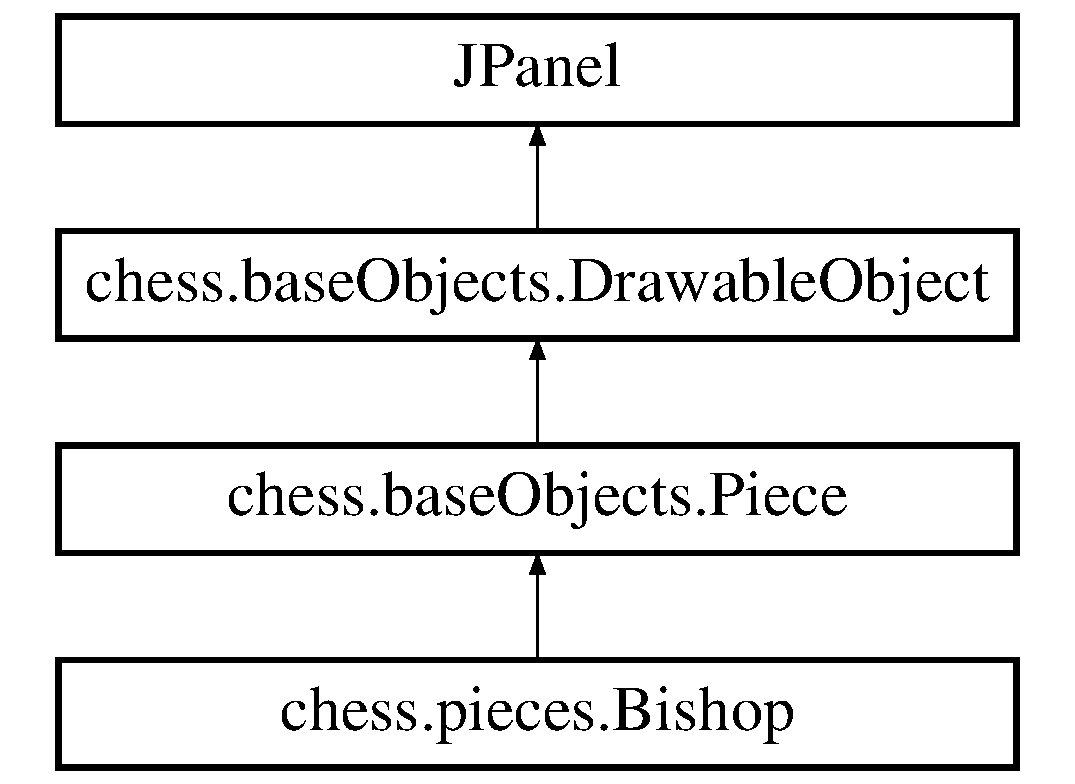
\includegraphics[height=4.000000cm]{classchess_1_1pieces_1_1_bishop}
\end{center}
\end{figure}
\subsection*{Public Member Functions}
\begin{DoxyCompactItemize}
\item 
{\bf Bishop} (String d)
\item 
void {\bf update\+Valid\+Destinations} ({\bf Board} board)
\item 
void {\bf render} (Graphics g)
\end{DoxyCompactItemize}
\subsection*{Additional Inherited Members}


\subsection{Constructor \& Destructor Documentation}
\index{chess\+::pieces\+::\+Bishop@{chess\+::pieces\+::\+Bishop}!Bishop@{Bishop}}
\index{Bishop@{Bishop}!chess\+::pieces\+::\+Bishop@{chess\+::pieces\+::\+Bishop}}
\subsubsection[{Bishop}]{\setlength{\rightskip}{0pt plus 5cm}chess.\+pieces.\+Bishop.\+Bishop (
\begin{DoxyParamCaption}
\item[{String}]{d}
\end{DoxyParamCaption}
)}\label{classchess_1_1pieces_1_1_bishop_a294419d7321521f10031faf9d92dd3c1}


\subsection{Member Function Documentation}
\index{chess\+::pieces\+::\+Bishop@{chess\+::pieces\+::\+Bishop}!render@{render}}
\index{render@{render}!chess\+::pieces\+::\+Bishop@{chess\+::pieces\+::\+Bishop}}
\subsubsection[{render}]{\setlength{\rightskip}{0pt plus 5cm}void chess.\+pieces.\+Bishop.\+render (
\begin{DoxyParamCaption}
\item[{Graphics}]{g}
\end{DoxyParamCaption}
)}\label{classchess_1_1pieces_1_1_bishop_a768b1596ac2d4d04f5c1d2d869f2ba28}
\index{chess\+::pieces\+::\+Bishop@{chess\+::pieces\+::\+Bishop}!update\+Valid\+Destinations@{update\+Valid\+Destinations}}
\index{update\+Valid\+Destinations@{update\+Valid\+Destinations}!chess\+::pieces\+::\+Bishop@{chess\+::pieces\+::\+Bishop}}
\subsubsection[{update\+Valid\+Destinations}]{\setlength{\rightskip}{0pt plus 5cm}void chess.\+pieces.\+Bishop.\+update\+Valid\+Destinations (
\begin{DoxyParamCaption}
\item[{{\bf Board}}]{board}
\end{DoxyParamCaption}
)}\label{classchess_1_1pieces_1_1_bishop_a0685f1c9fbd4571b65e6f0153935f751}


The documentation for this class was generated from the following file\+:\begin{DoxyCompactItemize}
\item 
src/chess/pieces/{\bf Bishop.\+java}\end{DoxyCompactItemize}

\section{chess.\+base\+Objects.\+Board Class Reference}
\label{classchess_1_1base_objects_1_1_board}\index{chess.\+base\+Objects.\+Board@{chess.\+base\+Objects.\+Board}}
\subsection*{Classes}
\begin{DoxyCompactItemize}
\item 
class {\bf Chess\+Board\+Cell\+Renderer}
\end{DoxyCompactItemize}
\subsection*{Public Member Functions}
\begin{DoxyCompactItemize}
\item 
{\bf Board} (int w, int h)
\item 
int {\bf get\+Width} ()
\item 
int {\bf get\+Height} ()
\item 
J\+Panel {\bf get\+Canvas} ()
\item 
{\bf Square} {\bf chess\+Get\+Square\+At} (int col, int row)
\item 
void {\bf set\+Piece\+At} ({\bf Piece} p, int col, int row)
\end{DoxyCompactItemize}


\subsection{Constructor \& Destructor Documentation}
\index{chess\+::base\+Objects\+::\+Board@{chess\+::base\+Objects\+::\+Board}!Board@{Board}}
\index{Board@{Board}!chess\+::base\+Objects\+::\+Board@{chess\+::base\+Objects\+::\+Board}}
\subsubsection[{Board}]{\setlength{\rightskip}{0pt plus 5cm}chess.\+base\+Objects.\+Board.\+Board (
\begin{DoxyParamCaption}
\item[{int}]{w, }
\item[{int}]{h}
\end{DoxyParamCaption}
)}\label{classchess_1_1base_objects_1_1_board_a8b9c1a12e57c92e39c7164badf7689b8}


\subsection{Member Function Documentation}
\index{chess\+::base\+Objects\+::\+Board@{chess\+::base\+Objects\+::\+Board}!chess\+Get\+Square\+At@{chess\+Get\+Square\+At}}
\index{chess\+Get\+Square\+At@{chess\+Get\+Square\+At}!chess\+::base\+Objects\+::\+Board@{chess\+::base\+Objects\+::\+Board}}
\subsubsection[{chess\+Get\+Square\+At}]{\setlength{\rightskip}{0pt plus 5cm}{\bf Square} chess.\+base\+Objects.\+Board.\+chess\+Get\+Square\+At (
\begin{DoxyParamCaption}
\item[{int}]{col, }
\item[{int}]{row}
\end{DoxyParamCaption}
)}\label{classchess_1_1base_objects_1_1_board_af144165033a4f3a95b7c357ed7d57a64}
Returns the square at the coordinates passed. Format = (x, y) = (col, row). Does check for boundary conditions. Rotates the axis so that (0, 0) means the bottom left instead of top right This is the Chess style of numbering


\begin{DoxyParams}{Parameters}
{\em col} & the x coordinate of the required square \\
\hline
{\em row} & the y coordinate of the required square \\
\hline
\end{DoxyParams}
\begin{DoxyReturn}{Returns}
the square at (col, row) if valid. Otherwise null. 
\end{DoxyReturn}
\index{chess\+::base\+Objects\+::\+Board@{chess\+::base\+Objects\+::\+Board}!get\+Canvas@{get\+Canvas}}
\index{get\+Canvas@{get\+Canvas}!chess\+::base\+Objects\+::\+Board@{chess\+::base\+Objects\+::\+Board}}
\subsubsection[{get\+Canvas}]{\setlength{\rightskip}{0pt plus 5cm}J\+Panel chess.\+base\+Objects.\+Board.\+get\+Canvas (
\begin{DoxyParamCaption}
{}
\end{DoxyParamCaption}
)}\label{classchess_1_1base_objects_1_1_board_af7113ee016011341070ecbd61adb8f3d}
\index{chess\+::base\+Objects\+::\+Board@{chess\+::base\+Objects\+::\+Board}!get\+Height@{get\+Height}}
\index{get\+Height@{get\+Height}!chess\+::base\+Objects\+::\+Board@{chess\+::base\+Objects\+::\+Board}}
\subsubsection[{get\+Height}]{\setlength{\rightskip}{0pt plus 5cm}int chess.\+base\+Objects.\+Board.\+get\+Height (
\begin{DoxyParamCaption}
{}
\end{DoxyParamCaption}
)}\label{classchess_1_1base_objects_1_1_board_ad519701abd9ea4ea06df06aa3c15aea9}
\index{chess\+::base\+Objects\+::\+Board@{chess\+::base\+Objects\+::\+Board}!get\+Width@{get\+Width}}
\index{get\+Width@{get\+Width}!chess\+::base\+Objects\+::\+Board@{chess\+::base\+Objects\+::\+Board}}
\subsubsection[{get\+Width}]{\setlength{\rightskip}{0pt plus 5cm}int chess.\+base\+Objects.\+Board.\+get\+Width (
\begin{DoxyParamCaption}
{}
\end{DoxyParamCaption}
)}\label{classchess_1_1base_objects_1_1_board_a2f8a5be3205b816926a0041f00abd75b}
\index{chess\+::base\+Objects\+::\+Board@{chess\+::base\+Objects\+::\+Board}!set\+Piece\+At@{set\+Piece\+At}}
\index{set\+Piece\+At@{set\+Piece\+At}!chess\+::base\+Objects\+::\+Board@{chess\+::base\+Objects\+::\+Board}}
\subsubsection[{set\+Piece\+At}]{\setlength{\rightskip}{0pt plus 5cm}void chess.\+base\+Objects.\+Board.\+set\+Piece\+At (
\begin{DoxyParamCaption}
\item[{{\bf Piece}}]{p, }
\item[{int}]{col, }
\item[{int}]{row}
\end{DoxyParamCaption}
)}\label{classchess_1_1base_objects_1_1_board_a0b7a9f450ef5bdfd782e7e180d8f83fc}


The documentation for this class was generated from the following file\+:\begin{DoxyCompactItemize}
\item 
src/chess/base\+Objects/{\bf Board.\+java}\end{DoxyCompactItemize}

\section{chess.\+base\+Objects.\+Board.\+Chess\+Board\+Cell\+Renderer Class Reference}
\label{classchess_1_1base_objects_1_1_board_1_1_chess_board_cell_renderer}\index{chess.\+base\+Objects.\+Board.\+Chess\+Board\+Cell\+Renderer@{chess.\+base\+Objects.\+Board.\+Chess\+Board\+Cell\+Renderer}}
Inheritance diagram for chess.\+base\+Objects.\+Board.\+Chess\+Board\+Cell\+Renderer\+:\begin{figure}[H]
\begin{center}
\leavevmode
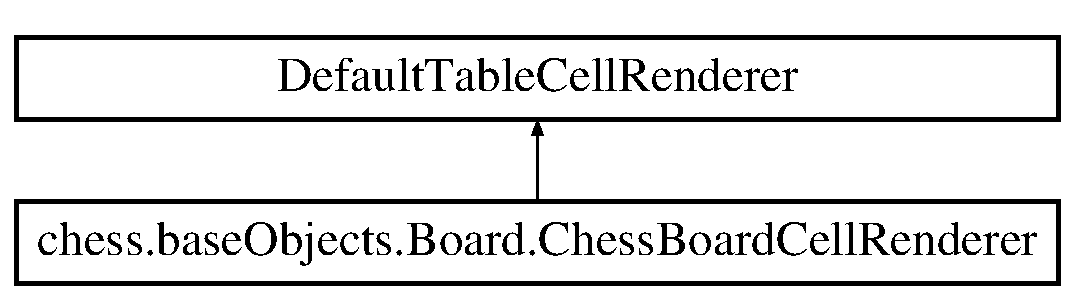
\includegraphics[height=2.000000cm]{classchess_1_1base_objects_1_1_board_1_1_chess_board_cell_renderer}
\end{center}
\end{figure}
\subsection*{Public Member Functions}
\begin{DoxyCompactItemize}
\item 
Component {\bf get\+Table\+Cell\+Renderer\+Component} (J\+Table table, Object value, boolean selected, boolean focused, int row, int column)
\end{DoxyCompactItemize}


\subsection{Member Function Documentation}
\index{chess\+::base\+Objects\+::\+Board\+::\+Chess\+Board\+Cell\+Renderer@{chess\+::base\+Objects\+::\+Board\+::\+Chess\+Board\+Cell\+Renderer}!get\+Table\+Cell\+Renderer\+Component@{get\+Table\+Cell\+Renderer\+Component}}
\index{get\+Table\+Cell\+Renderer\+Component@{get\+Table\+Cell\+Renderer\+Component}!chess\+::base\+Objects\+::\+Board\+::\+Chess\+Board\+Cell\+Renderer@{chess\+::base\+Objects\+::\+Board\+::\+Chess\+Board\+Cell\+Renderer}}
\subsubsection[{get\+Table\+Cell\+Renderer\+Component}]{\setlength{\rightskip}{0pt plus 5cm}Component chess.\+base\+Objects.\+Board.\+Chess\+Board\+Cell\+Renderer.\+get\+Table\+Cell\+Renderer\+Component (
\begin{DoxyParamCaption}
\item[{J\+Table}]{table, }
\item[{Object}]{value, }
\item[{boolean}]{selected, }
\item[{boolean}]{focused, }
\item[{int}]{row, }
\item[{int}]{column}
\end{DoxyParamCaption}
)}\label{classchess_1_1base_objects_1_1_board_1_1_chess_board_cell_renderer_a5b781b15b1ba40bf0665ab95665853af}


The documentation for this class was generated from the following file\+:\begin{DoxyCompactItemize}
\item 
src/chess/base\+Objects/{\bf Board.\+java}\end{DoxyCompactItemize}

\section{chess.\+gamemodes.\+Classic\+Chess Class Reference}
\label{classchess_1_1gamemodes_1_1_classic_chess}\index{chess.\+gamemodes.\+Classic\+Chess@{chess.\+gamemodes.\+Classic\+Chess}}
Inheritance diagram for chess.\+gamemodes.\+Classic\+Chess\+:\begin{figure}[H]
\begin{center}
\leavevmode
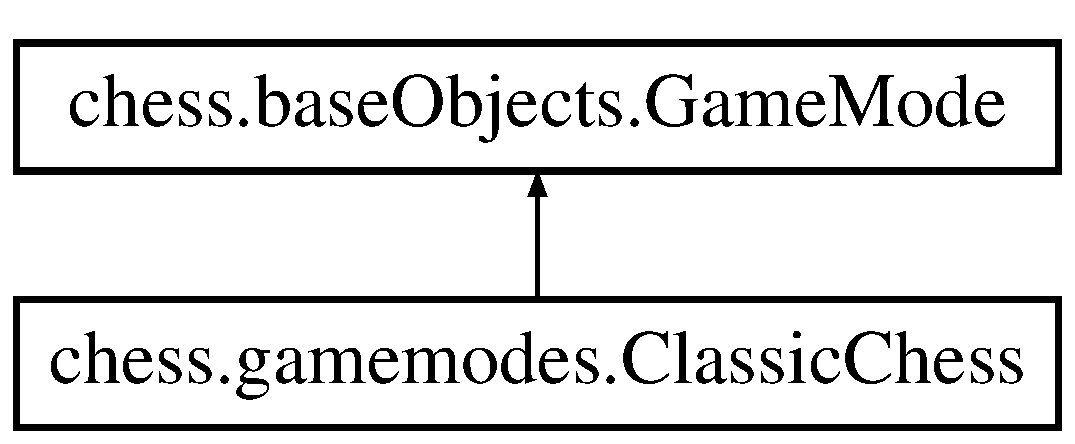
\includegraphics[height=2.000000cm]{classchess_1_1gamemodes_1_1_classic_chess}
\end{center}
\end{figure}
\subsection*{Public Member Functions}
\begin{DoxyCompactItemize}
\item 
{\bf Classic\+Chess} ()
\end{DoxyCompactItemize}
\subsection*{Additional Inherited Members}


\subsection{Constructor \& Destructor Documentation}
\index{chess\+::gamemodes\+::\+Classic\+Chess@{chess\+::gamemodes\+::\+Classic\+Chess}!Classic\+Chess@{Classic\+Chess}}
\index{Classic\+Chess@{Classic\+Chess}!chess\+::gamemodes\+::\+Classic\+Chess@{chess\+::gamemodes\+::\+Classic\+Chess}}
\subsubsection[{Classic\+Chess}]{\setlength{\rightskip}{0pt plus 5cm}chess.\+gamemodes.\+Classic\+Chess.\+Classic\+Chess (
\begin{DoxyParamCaption}
{}
\end{DoxyParamCaption}
)}\label{classchess_1_1gamemodes_1_1_classic_chess_a8651b004542217834ea885fabb0cea9e}


The documentation for this class was generated from the following file\+:\begin{DoxyCompactItemize}
\item 
src/chess/gamemodes/{\bf Classic\+Chess.\+java}\end{DoxyCompactItemize}

\section{chess.\+base\+Objects.\+Drawable\+Object Class Reference}
\label{classchess_1_1base_objects_1_1_drawable_object}\index{chess.\+base\+Objects.\+Drawable\+Object@{chess.\+base\+Objects.\+Drawable\+Object}}
Inheritance diagram for chess.\+base\+Objects.\+Drawable\+Object\+:\begin{figure}[H]
\begin{center}
\leavevmode
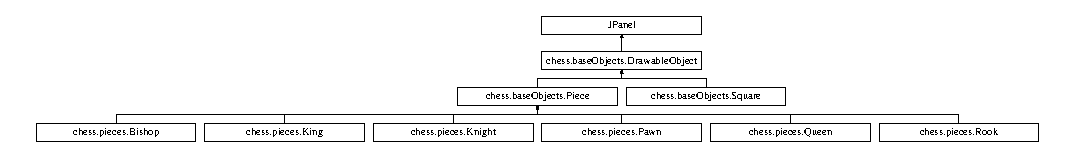
\includegraphics[height=1.681682cm]{classchess_1_1base_objects_1_1_drawable_object}
\end{center}
\end{figure}
\subsection*{Public Member Functions}
\begin{DoxyCompactItemize}
\item 
{\bf Drawable\+Object} ()
\item 
abstract void {\bf render} (Graphics g)
\item 
void {\bf paint} (Graphics g)
\end{DoxyCompactItemize}


\subsection{Constructor \& Destructor Documentation}
\index{chess\+::base\+Objects\+::\+Drawable\+Object@{chess\+::base\+Objects\+::\+Drawable\+Object}!Drawable\+Object@{Drawable\+Object}}
\index{Drawable\+Object@{Drawable\+Object}!chess\+::base\+Objects\+::\+Drawable\+Object@{chess\+::base\+Objects\+::\+Drawable\+Object}}
\subsubsection[{Drawable\+Object}]{\setlength{\rightskip}{0pt plus 5cm}chess.\+base\+Objects.\+Drawable\+Object.\+Drawable\+Object (
\begin{DoxyParamCaption}
{}
\end{DoxyParamCaption}
)}\label{classchess_1_1base_objects_1_1_drawable_object_ae12c51f3140526e22adcaeb21c9e8b1a}


\subsection{Member Function Documentation}
\index{chess\+::base\+Objects\+::\+Drawable\+Object@{chess\+::base\+Objects\+::\+Drawable\+Object}!paint@{paint}}
\index{paint@{paint}!chess\+::base\+Objects\+::\+Drawable\+Object@{chess\+::base\+Objects\+::\+Drawable\+Object}}
\subsubsection[{paint}]{\setlength{\rightskip}{0pt plus 5cm}void chess.\+base\+Objects.\+Drawable\+Object.\+paint (
\begin{DoxyParamCaption}
\item[{Graphics}]{g}
\end{DoxyParamCaption}
)}\label{classchess_1_1base_objects_1_1_drawable_object_a18cda4a7ba656e6093288fc3d771ee88}
\index{chess\+::base\+Objects\+::\+Drawable\+Object@{chess\+::base\+Objects\+::\+Drawable\+Object}!render@{render}}
\index{render@{render}!chess\+::base\+Objects\+::\+Drawable\+Object@{chess\+::base\+Objects\+::\+Drawable\+Object}}
\subsubsection[{render}]{\setlength{\rightskip}{0pt plus 5cm}abstract void chess.\+base\+Objects.\+Drawable\+Object.\+render (
\begin{DoxyParamCaption}
\item[{Graphics}]{g}
\end{DoxyParamCaption}
)\hspace{0.3cm}{\ttfamily [abstract]}}\label{classchess_1_1base_objects_1_1_drawable_object_ad011e9882e50f370dfc5a13511bdab1b}


The documentation for this class was generated from the following file\+:\begin{DoxyCompactItemize}
\item 
src/chess/base\+Objects/{\bf Drawable\+Object.\+java}\end{DoxyCompactItemize}

\section{chess.\+base\+Objects.\+Event Class Reference}
\label{classchess_1_1base_objects_1_1_event}\index{chess.\+base\+Objects.\+Event@{chess.\+base\+Objects.\+Event}}
\subsection*{Classes}
\begin{DoxyCompactItemize}
\item 
enum {\bfseries Event\+Type}
\end{DoxyCompactItemize}


The documentation for this class was generated from the following file\+:\begin{DoxyCompactItemize}
\item 
src/chess/base\+Objects/{\bf Event.\+java}\end{DoxyCompactItemize}

\section{chess.\+custom.\+Faction Enum Reference}
\label{enumchess_1_1custom_1_1_faction}\index{chess.\+custom.\+Faction@{chess.\+custom.\+Faction}}
\subsection*{Public Attributes}
\begin{DoxyCompactItemize}
\item 
{\bf B\+L\+A\+C\+K}
\end{DoxyCompactItemize}


\subsection{Member Data Documentation}
\index{chess\+::custom\+::\+Faction@{chess\+::custom\+::\+Faction}!B\+L\+A\+C\+K@{B\+L\+A\+C\+K}}
\index{B\+L\+A\+C\+K@{B\+L\+A\+C\+K}!chess\+::custom\+::\+Faction@{chess\+::custom\+::\+Faction}}
\subsubsection[{B\+L\+A\+C\+K}]{\setlength{\rightskip}{0pt plus 5cm}chess.\+custom.\+Faction.\+B\+L\+A\+C\+K}\label{enumchess_1_1custom_1_1_faction_ae494d05789ce12f1f8937300f14e093f}


The documentation for this enum was generated from the following file\+:\begin{DoxyCompactItemize}
\item 
src/chess/custom/{\bf Faction.\+java}\end{DoxyCompactItemize}

\section{chess.\+base\+Objects.\+Game Class Reference}
\label{classchess_1_1base_objects_1_1_game}\index{chess.\+base\+Objects.\+Game@{chess.\+base\+Objects.\+Game}}
\subsection*{Public Member Functions}
\begin{DoxyCompactItemize}
\item 
{\bf Game} ({\bf Game\+Mode} \+\_\+mode)
\item 
{\bf History} {\bf get\+History} ()
\item 
{\bf Game\+Mode} {\bf get\+Mode} ()
\item 
J\+Panel {\bf get\+Canvas} ()
\end{DoxyCompactItemize}


\subsection{Constructor \& Destructor Documentation}
\index{chess\+::base\+Objects\+::\+Game@{chess\+::base\+Objects\+::\+Game}!Game@{Game}}
\index{Game@{Game}!chess\+::base\+Objects\+::\+Game@{chess\+::base\+Objects\+::\+Game}}
\subsubsection[{Game}]{\setlength{\rightskip}{0pt plus 5cm}chess.\+base\+Objects.\+Game.\+Game (
\begin{DoxyParamCaption}
\item[{{\bf Game\+Mode}}]{\+\_\+mode}
\end{DoxyParamCaption}
)}\label{classchess_1_1base_objects_1_1_game_ab47fd3d548eaebc06bd4d4c2de3dc5c9}


\subsection{Member Function Documentation}
\index{chess\+::base\+Objects\+::\+Game@{chess\+::base\+Objects\+::\+Game}!get\+Canvas@{get\+Canvas}}
\index{get\+Canvas@{get\+Canvas}!chess\+::base\+Objects\+::\+Game@{chess\+::base\+Objects\+::\+Game}}
\subsubsection[{get\+Canvas}]{\setlength{\rightskip}{0pt plus 5cm}J\+Panel chess.\+base\+Objects.\+Game.\+get\+Canvas (
\begin{DoxyParamCaption}
{}
\end{DoxyParamCaption}
)}\label{classchess_1_1base_objects_1_1_game_a7ca906a2d5600fc892ed531787d966c0}
\index{chess\+::base\+Objects\+::\+Game@{chess\+::base\+Objects\+::\+Game}!get\+History@{get\+History}}
\index{get\+History@{get\+History}!chess\+::base\+Objects\+::\+Game@{chess\+::base\+Objects\+::\+Game}}
\subsubsection[{get\+History}]{\setlength{\rightskip}{0pt plus 5cm}{\bf History} chess.\+base\+Objects.\+Game.\+get\+History (
\begin{DoxyParamCaption}
{}
\end{DoxyParamCaption}
)}\label{classchess_1_1base_objects_1_1_game_ac27f7a5d85b5daa5a27bae403832a25c}
\index{chess\+::base\+Objects\+::\+Game@{chess\+::base\+Objects\+::\+Game}!get\+Mode@{get\+Mode}}
\index{get\+Mode@{get\+Mode}!chess\+::base\+Objects\+::\+Game@{chess\+::base\+Objects\+::\+Game}}
\subsubsection[{get\+Mode}]{\setlength{\rightskip}{0pt plus 5cm}{\bf Game\+Mode} chess.\+base\+Objects.\+Game.\+get\+Mode (
\begin{DoxyParamCaption}
{}
\end{DoxyParamCaption}
)}\label{classchess_1_1base_objects_1_1_game_a94ffad44a168a30e7f4c95024b84897b}


The documentation for this class was generated from the following file\+:\begin{DoxyCompactItemize}
\item 
src/chess/base\+Objects/{\bf Game.\+java}\end{DoxyCompactItemize}

\section{chess.\+base\+Objects.\+Game\+Mode Class Reference}
\label{classchess_1_1base_objects_1_1_game_mode}\index{chess.\+base\+Objects.\+Game\+Mode@{chess.\+base\+Objects.\+Game\+Mode}}
Inheritance diagram for chess.\+base\+Objects.\+Game\+Mode\+:\begin{figure}[H]
\begin{center}
\leavevmode
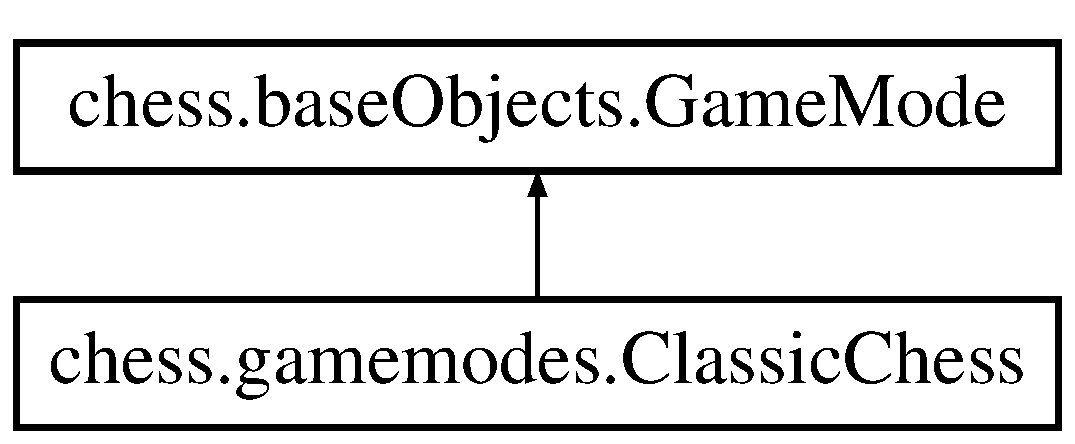
\includegraphics[height=2.000000cm]{classchess_1_1base_objects_1_1_game_mode}
\end{center}
\end{figure}
\subsection*{Public Member Functions}
\begin{DoxyCompactItemize}
\item 
{\bf Player} {\bf get\+Next\+Active\+Player} ()
\item 
{\bf Game\+Mode} (int \+\_\+num\+Teams, int[$\,$] num\+Players\+In\+Teams)
\item 
J\+Panel {\bf get\+Canvas} ()
\end{DoxyCompactItemize}
\subsection*{Protected Member Functions}
\begin{DoxyCompactItemize}
\item 
void {\bf set\+Piece\+At} (char c, int col, int row)
\end{DoxyCompactItemize}
\subsection*{Protected Attributes}
\begin{DoxyCompactItemize}
\item 
{\bf Board} {\bf board}
\end{DoxyCompactItemize}


\subsection{Detailed Description}
Class that keeps track of the various teams, the board and the turn order. why is board in this class? 

\subsection{Constructor \& Destructor Documentation}
\index{chess\+::base\+Objects\+::\+Game\+Mode@{chess\+::base\+Objects\+::\+Game\+Mode}!Game\+Mode@{Game\+Mode}}
\index{Game\+Mode@{Game\+Mode}!chess\+::base\+Objects\+::\+Game\+Mode@{chess\+::base\+Objects\+::\+Game\+Mode}}
\subsubsection[{Game\+Mode}]{\setlength{\rightskip}{0pt plus 5cm}chess.\+base\+Objects.\+Game\+Mode.\+Game\+Mode (
\begin{DoxyParamCaption}
\item[{int}]{\+\_\+num\+Teams, }
\item[{int[$\,$]}]{num\+Players\+In\+Teams}
\end{DoxyParamCaption}
)}\label{classchess_1_1base_objects_1_1_game_mode_aa222fc4c57f80dc054fafeb060bc62a9}


\subsection{Member Function Documentation}
\index{chess\+::base\+Objects\+::\+Game\+Mode@{chess\+::base\+Objects\+::\+Game\+Mode}!get\+Canvas@{get\+Canvas}}
\index{get\+Canvas@{get\+Canvas}!chess\+::base\+Objects\+::\+Game\+Mode@{chess\+::base\+Objects\+::\+Game\+Mode}}
\subsubsection[{get\+Canvas}]{\setlength{\rightskip}{0pt plus 5cm}J\+Panel chess.\+base\+Objects.\+Game\+Mode.\+get\+Canvas (
\begin{DoxyParamCaption}
{}
\end{DoxyParamCaption}
)}\label{classchess_1_1base_objects_1_1_game_mode_a462da7c37d042a4ebd2e6c9f8c70e348}
\index{chess\+::base\+Objects\+::\+Game\+Mode@{chess\+::base\+Objects\+::\+Game\+Mode}!get\+Next\+Active\+Player@{get\+Next\+Active\+Player}}
\index{get\+Next\+Active\+Player@{get\+Next\+Active\+Player}!chess\+::base\+Objects\+::\+Game\+Mode@{chess\+::base\+Objects\+::\+Game\+Mode}}
\subsubsection[{get\+Next\+Active\+Player}]{\setlength{\rightskip}{0pt plus 5cm}{\bf Player} chess.\+base\+Objects.\+Game\+Mode.\+get\+Next\+Active\+Player (
\begin{DoxyParamCaption}
{}
\end{DoxyParamCaption}
)}\label{classchess_1_1base_objects_1_1_game_mode_a675c0ba0fe91bbc23deff859c3609fca}
\index{chess\+::base\+Objects\+::\+Game\+Mode@{chess\+::base\+Objects\+::\+Game\+Mode}!set\+Piece\+At@{set\+Piece\+At}}
\index{set\+Piece\+At@{set\+Piece\+At}!chess\+::base\+Objects\+::\+Game\+Mode@{chess\+::base\+Objects\+::\+Game\+Mode}}
\subsubsection[{set\+Piece\+At}]{\setlength{\rightskip}{0pt plus 5cm}void chess.\+base\+Objects.\+Game\+Mode.\+set\+Piece\+At (
\begin{DoxyParamCaption}
\item[{char}]{c, }
\item[{int}]{col, }
\item[{int}]{row}
\end{DoxyParamCaption}
)\hspace{0.3cm}{\ttfamily [protected]}}\label{classchess_1_1base_objects_1_1_game_mode_a555926a325322202df03b2e89421bb02}


\subsection{Member Data Documentation}
\index{chess\+::base\+Objects\+::\+Game\+Mode@{chess\+::base\+Objects\+::\+Game\+Mode}!board@{board}}
\index{board@{board}!chess\+::base\+Objects\+::\+Game\+Mode@{chess\+::base\+Objects\+::\+Game\+Mode}}
\subsubsection[{board}]{\setlength{\rightskip}{0pt plus 5cm}{\bf Board} chess.\+base\+Objects.\+Game\+Mode.\+board\hspace{0.3cm}{\ttfamily [protected]}}\label{classchess_1_1base_objects_1_1_game_mode_a78fbd210f186558554b8e9e0879dc6c6}


The documentation for this class was generated from the following file\+:\begin{DoxyCompactItemize}
\item 
src/chess/base\+Objects/{\bf Game\+Mode.\+java}\end{DoxyCompactItemize}

\section{chess.\+base\+Objects.\+History Class Reference}
\label{classchess_1_1base_objects_1_1_history}\index{chess.\+base\+Objects.\+History@{chess.\+base\+Objects.\+History}}


The documentation for this class was generated from the following file\+:\begin{DoxyCompactItemize}
\item 
src/chess/base\+Objects/{\bf History.\+java}\end{DoxyCompactItemize}

\section{chess.\+pieces.\+King Class Reference}
\label{classchess_1_1pieces_1_1_king}\index{chess.\+pieces.\+King@{chess.\+pieces.\+King}}
Inheritance diagram for chess.\+pieces.\+King\+:\begin{figure}[H]
\begin{center}
\leavevmode
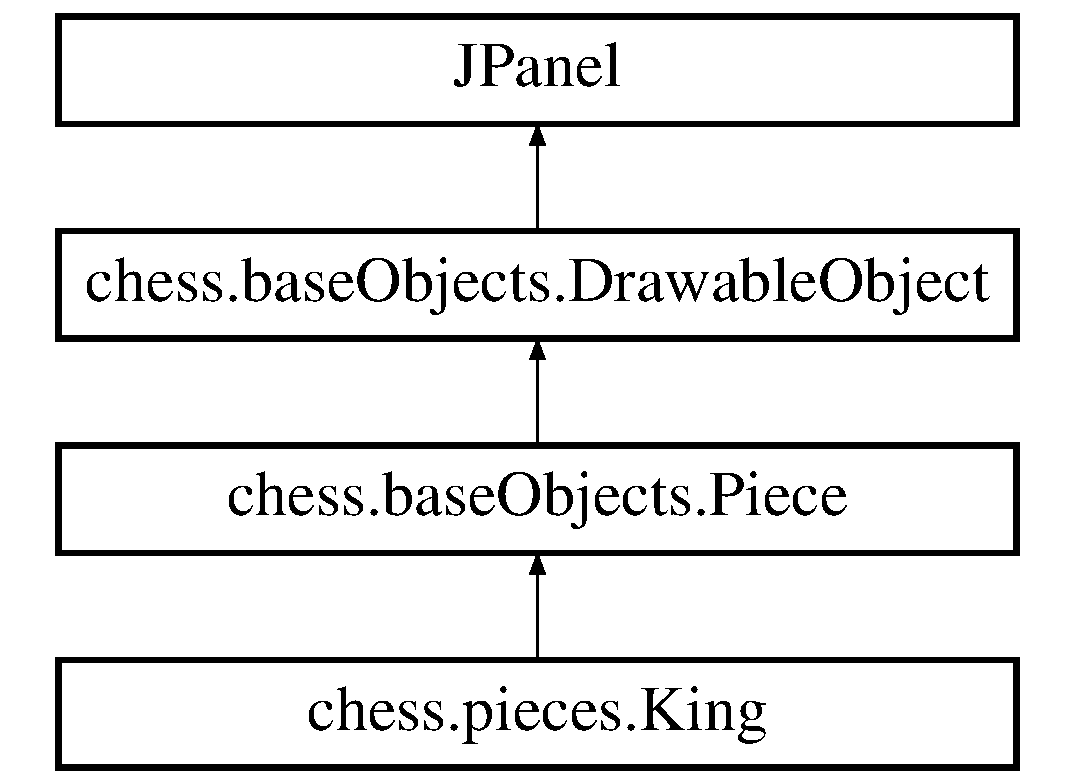
\includegraphics[height=4.000000cm]{classchess_1_1pieces_1_1_king}
\end{center}
\end{figure}
\subsection*{Public Member Functions}
\begin{DoxyCompactItemize}
\item 
{\bf King} (String d)
\item 
void {\bf update\+Valid\+Destinations} ({\bf Square}[$\,$][$\,$] board)
\item 
void {\bf update\+Valid\+Destinations} ({\bf Board} board)
\item 
void {\bf render} (Graphics g)
\end{DoxyCompactItemize}
\subsection*{Additional Inherited Members}


\subsection{Constructor \& Destructor Documentation}
\index{chess\+::pieces\+::\+King@{chess\+::pieces\+::\+King}!King@{King}}
\index{King@{King}!chess\+::pieces\+::\+King@{chess\+::pieces\+::\+King}}
\subsubsection[{King}]{\setlength{\rightskip}{0pt plus 5cm}chess.\+pieces.\+King.\+King (
\begin{DoxyParamCaption}
\item[{String}]{d}
\end{DoxyParamCaption}
)}\label{classchess_1_1pieces_1_1_king_a0bb5bc36ad555071141d663b118b7ec2}


\subsection{Member Function Documentation}
\index{chess\+::pieces\+::\+King@{chess\+::pieces\+::\+King}!render@{render}}
\index{render@{render}!chess\+::pieces\+::\+King@{chess\+::pieces\+::\+King}}
\subsubsection[{render}]{\setlength{\rightskip}{0pt plus 5cm}void chess.\+pieces.\+King.\+render (
\begin{DoxyParamCaption}
\item[{Graphics}]{g}
\end{DoxyParamCaption}
)}\label{classchess_1_1pieces_1_1_king_a030a95bf91e6bb5c9d70fccff5a7c8ed}
\index{chess\+::pieces\+::\+King@{chess\+::pieces\+::\+King}!update\+Valid\+Destinations@{update\+Valid\+Destinations}}
\index{update\+Valid\+Destinations@{update\+Valid\+Destinations}!chess\+::pieces\+::\+King@{chess\+::pieces\+::\+King}}
\subsubsection[{update\+Valid\+Destinations}]{\setlength{\rightskip}{0pt plus 5cm}void chess.\+pieces.\+King.\+update\+Valid\+Destinations (
\begin{DoxyParamCaption}
\item[{{\bf Square}}]{board[$\,$][$\,$]}
\end{DoxyParamCaption}
)}\label{classchess_1_1pieces_1_1_king_a9b7e16d1737711c0b2ce64e125927be7}
\index{chess\+::pieces\+::\+King@{chess\+::pieces\+::\+King}!update\+Valid\+Destinations@{update\+Valid\+Destinations}}
\index{update\+Valid\+Destinations@{update\+Valid\+Destinations}!chess\+::pieces\+::\+King@{chess\+::pieces\+::\+King}}
\subsubsection[{update\+Valid\+Destinations}]{\setlength{\rightskip}{0pt plus 5cm}void chess.\+pieces.\+King.\+update\+Valid\+Destinations (
\begin{DoxyParamCaption}
\item[{{\bf Board}}]{board}
\end{DoxyParamCaption}
)}\label{classchess_1_1pieces_1_1_king_a17c0a42263b73b87816b36d895cb9004}


The documentation for this class was generated from the following file\+:\begin{DoxyCompactItemize}
\item 
src/chess/pieces/{\bf King.\+java}\end{DoxyCompactItemize}

\section{chess.\+pieces.\+Knight Class Reference}
\label{classchess_1_1pieces_1_1_knight}\index{chess.\+pieces.\+Knight@{chess.\+pieces.\+Knight}}
Inheritance diagram for chess.\+pieces.\+Knight\+:\begin{figure}[H]
\begin{center}
\leavevmode
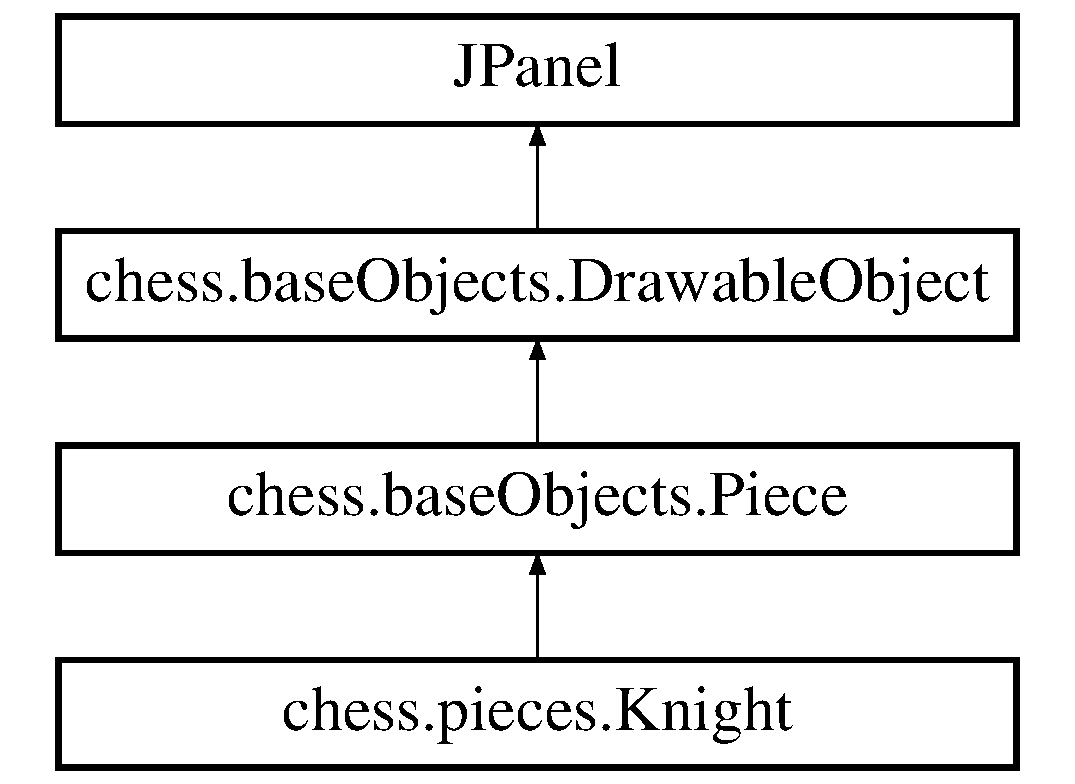
\includegraphics[height=4.000000cm]{classchess_1_1pieces_1_1_knight}
\end{center}
\end{figure}
\subsection*{Public Member Functions}
\begin{DoxyCompactItemize}
\item 
{\bf Knight} (String \+\_\+name)
\item 
void {\bf update\+Valid\+Destinations} ({\bf Square}[$\,$][$\,$] board)
\item 
void {\bf update\+Valid\+Destinations} ({\bf Board} board)
\item 
void {\bf render} (Graphics g)
\end{DoxyCompactItemize}
\subsection*{Additional Inherited Members}


\subsection{Constructor \& Destructor Documentation}
\index{chess\+::pieces\+::\+Knight@{chess\+::pieces\+::\+Knight}!Knight@{Knight}}
\index{Knight@{Knight}!chess\+::pieces\+::\+Knight@{chess\+::pieces\+::\+Knight}}
\subsubsection[{Knight}]{\setlength{\rightskip}{0pt plus 5cm}chess.\+pieces.\+Knight.\+Knight (
\begin{DoxyParamCaption}
\item[{String}]{\+\_\+name}
\end{DoxyParamCaption}
)}\label{classchess_1_1pieces_1_1_knight_ad879541a843b618e0ab8d8cbab59352b}


\subsection{Member Function Documentation}
\index{chess\+::pieces\+::\+Knight@{chess\+::pieces\+::\+Knight}!render@{render}}
\index{render@{render}!chess\+::pieces\+::\+Knight@{chess\+::pieces\+::\+Knight}}
\subsubsection[{render}]{\setlength{\rightskip}{0pt plus 5cm}void chess.\+pieces.\+Knight.\+render (
\begin{DoxyParamCaption}
\item[{Graphics}]{g}
\end{DoxyParamCaption}
)}\label{classchess_1_1pieces_1_1_knight_aabe2c447a9317a93b24e6f88eaac6429}
\index{chess\+::pieces\+::\+Knight@{chess\+::pieces\+::\+Knight}!update\+Valid\+Destinations@{update\+Valid\+Destinations}}
\index{update\+Valid\+Destinations@{update\+Valid\+Destinations}!chess\+::pieces\+::\+Knight@{chess\+::pieces\+::\+Knight}}
\subsubsection[{update\+Valid\+Destinations}]{\setlength{\rightskip}{0pt plus 5cm}void chess.\+pieces.\+Knight.\+update\+Valid\+Destinations (
\begin{DoxyParamCaption}
\item[{{\bf Square}}]{board[$\,$][$\,$]}
\end{DoxyParamCaption}
)}\label{classchess_1_1pieces_1_1_knight_ad112987a525be53841834871c34a6410}
\index{chess\+::pieces\+::\+Knight@{chess\+::pieces\+::\+Knight}!update\+Valid\+Destinations@{update\+Valid\+Destinations}}
\index{update\+Valid\+Destinations@{update\+Valid\+Destinations}!chess\+::pieces\+::\+Knight@{chess\+::pieces\+::\+Knight}}
\subsubsection[{update\+Valid\+Destinations}]{\setlength{\rightskip}{0pt plus 5cm}void chess.\+pieces.\+Knight.\+update\+Valid\+Destinations (
\begin{DoxyParamCaption}
\item[{{\bf Board}}]{board}
\end{DoxyParamCaption}
)}\label{classchess_1_1pieces_1_1_knight_a5464b92e15a86b25ed46067610cbe2e9}


The documentation for this class was generated from the following file\+:\begin{DoxyCompactItemize}
\item 
src/chess/pieces/{\bf Knight.\+java}\end{DoxyCompactItemize}

\section{chess.\+gui.\+Main\+Menu.\+Load\+Game\+Listener Class Reference}
\label{classchess_1_1gui_1_1_main_menu_1_1_load_game_listener}\index{chess.\+gui.\+Main\+Menu.\+Load\+Game\+Listener@{chess.\+gui.\+Main\+Menu.\+Load\+Game\+Listener}}
Inheritance diagram for chess.\+gui.\+Main\+Menu.\+Load\+Game\+Listener\+:\begin{figure}[H]
\begin{center}
\leavevmode
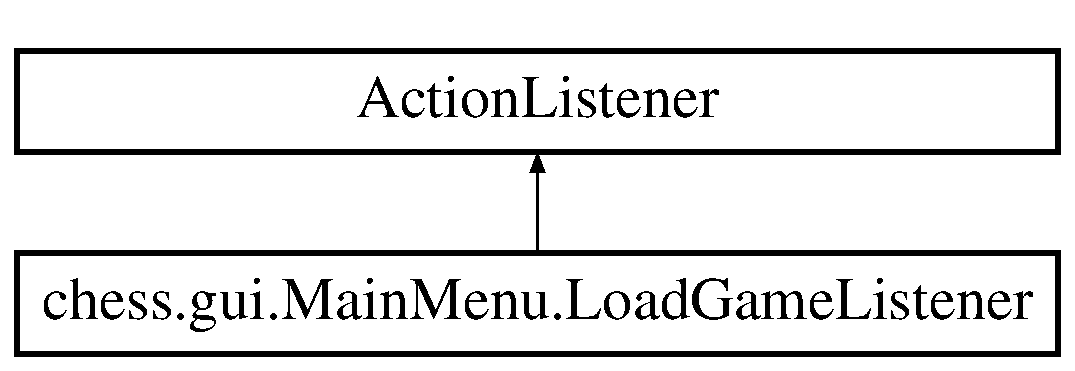
\includegraphics[height=2.000000cm]{classchess_1_1gui_1_1_main_menu_1_1_load_game_listener}
\end{center}
\end{figure}
\subsection*{Public Member Functions}
\begin{DoxyCompactItemize}
\item 
void {\bf action\+Performed} (Action\+Event action\+Event)
\end{DoxyCompactItemize}


\subsection{Member Function Documentation}
\index{chess\+::gui\+::\+Main\+Menu\+::\+Load\+Game\+Listener@{chess\+::gui\+::\+Main\+Menu\+::\+Load\+Game\+Listener}!action\+Performed@{action\+Performed}}
\index{action\+Performed@{action\+Performed}!chess\+::gui\+::\+Main\+Menu\+::\+Load\+Game\+Listener@{chess\+::gui\+::\+Main\+Menu\+::\+Load\+Game\+Listener}}
\subsubsection[{action\+Performed}]{\setlength{\rightskip}{0pt plus 5cm}void chess.\+gui.\+Main\+Menu.\+Load\+Game\+Listener.\+action\+Performed (
\begin{DoxyParamCaption}
\item[{Action\+Event}]{action\+Event}
\end{DoxyParamCaption}
)}\label{classchess_1_1gui_1_1_main_menu_1_1_load_game_listener_ad22ba94c86f1ac2c984831ca2d97c6d9}


The documentation for this class was generated from the following file\+:\begin{DoxyCompactItemize}
\item 
src/chess/gui/{\bf Main\+Menu.\+java}\end{DoxyCompactItemize}

\section{chess.\+gui.\+Main\+Menu Class Reference}
\label{classchess_1_1gui_1_1_main_menu}\index{chess.\+gui.\+Main\+Menu@{chess.\+gui.\+Main\+Menu}}
\subsection*{Classes}
\begin{DoxyCompactItemize}
\item 
class {\bf Load\+Game\+Listener}
\item 
class {\bf New\+Game\+Listener}
\item 
class {\bf Quit\+Listener}
\item 
class {\bf Settings\+Listener}
\end{DoxyCompactItemize}
\subsection*{Public Member Functions}
\begin{DoxyCompactItemize}
\item 
{\bf Main\+Menu} ()
\end{DoxyCompactItemize}


\subsection{Detailed Description}
Created by Fez on 9/15/14. 

\subsection{Constructor \& Destructor Documentation}
\index{chess\+::gui\+::\+Main\+Menu@{chess\+::gui\+::\+Main\+Menu}!Main\+Menu@{Main\+Menu}}
\index{Main\+Menu@{Main\+Menu}!chess\+::gui\+::\+Main\+Menu@{chess\+::gui\+::\+Main\+Menu}}
\subsubsection[{Main\+Menu}]{\setlength{\rightskip}{0pt plus 5cm}chess.\+gui.\+Main\+Menu.\+Main\+Menu (
\begin{DoxyParamCaption}
{}
\end{DoxyParamCaption}
)}\label{classchess_1_1gui_1_1_main_menu_aaad463683517f394f811b8d5945b9b44}


The documentation for this class was generated from the following file\+:\begin{DoxyCompactItemize}
\item 
src/chess/gui/{\bf Main\+Menu.\+java}\end{DoxyCompactItemize}

\section{chess.\+base\+Objects.\+Move\+Style Class Reference}
\label{classchess_1_1base_objects_1_1_move_style}\index{chess.\+base\+Objects.\+Move\+Style@{chess.\+base\+Objects.\+Move\+Style}}
\subsection*{Public Member Functions}
\begin{DoxyCompactItemize}
\item 
{\bf Move\+Style} (int \+\_\+dx, int \+\_\+dy, boolean \+\_\+collides\+During, boolean \+\_\+collides\+At\+End, boolean \+\_\+kill\+Only, boolean[$\,$] \+\_\+infinite\+Move)
\item 
int {\bf get\+Dx} ()
\item 
int {\bf get\+Dy} ()
\item 
boolean {\bf does\+Collide\+During} ()
\item 
boolean {\bf does\+Collide\+At\+End} ()
\item 
Set$<$ {\bf Square} $>$ {\bf get\+Possible\+Destinations} ({\bf Board} board, {\bf Piece} p)
\item 
boolean {\bf is\+Kill\+Only} ()
\end{DoxyCompactItemize}


\subsection{Constructor \& Destructor Documentation}
\index{chess\+::base\+Objects\+::\+Move\+Style@{chess\+::base\+Objects\+::\+Move\+Style}!Move\+Style@{Move\+Style}}
\index{Move\+Style@{Move\+Style}!chess\+::base\+Objects\+::\+Move\+Style@{chess\+::base\+Objects\+::\+Move\+Style}}
\subsubsection[{Move\+Style}]{\setlength{\rightskip}{0pt plus 5cm}chess.\+base\+Objects.\+Move\+Style.\+Move\+Style (
\begin{DoxyParamCaption}
\item[{int}]{\+\_\+dx, }
\item[{int}]{\+\_\+dy, }
\item[{boolean}]{\+\_\+collides\+During, }
\item[{boolean}]{\+\_\+collides\+At\+End, }
\item[{boolean}]{\+\_\+kill\+Only, }
\item[{boolean[$\,$]}]{\+\_\+infinite\+Move}
\end{DoxyParamCaption}
)}\label{classchess_1_1base_objects_1_1_move_style_a8a0cf207547aed128ef36dc8a25c3dc7}


\subsection{Member Function Documentation}
\index{chess\+::base\+Objects\+::\+Move\+Style@{chess\+::base\+Objects\+::\+Move\+Style}!does\+Collide\+At\+End@{does\+Collide\+At\+End}}
\index{does\+Collide\+At\+End@{does\+Collide\+At\+End}!chess\+::base\+Objects\+::\+Move\+Style@{chess\+::base\+Objects\+::\+Move\+Style}}
\subsubsection[{does\+Collide\+At\+End}]{\setlength{\rightskip}{0pt plus 5cm}boolean chess.\+base\+Objects.\+Move\+Style.\+does\+Collide\+At\+End (
\begin{DoxyParamCaption}
{}
\end{DoxyParamCaption}
)}\label{classchess_1_1base_objects_1_1_move_style_a2c06aeec1d03c24ac5838d9dc9381f37}
\index{chess\+::base\+Objects\+::\+Move\+Style@{chess\+::base\+Objects\+::\+Move\+Style}!does\+Collide\+During@{does\+Collide\+During}}
\index{does\+Collide\+During@{does\+Collide\+During}!chess\+::base\+Objects\+::\+Move\+Style@{chess\+::base\+Objects\+::\+Move\+Style}}
\subsubsection[{does\+Collide\+During}]{\setlength{\rightskip}{0pt plus 5cm}boolean chess.\+base\+Objects.\+Move\+Style.\+does\+Collide\+During (
\begin{DoxyParamCaption}
{}
\end{DoxyParamCaption}
)}\label{classchess_1_1base_objects_1_1_move_style_a1d00923443a40a17ed8fe31c6e839e79}
\index{chess\+::base\+Objects\+::\+Move\+Style@{chess\+::base\+Objects\+::\+Move\+Style}!get\+Dx@{get\+Dx}}
\index{get\+Dx@{get\+Dx}!chess\+::base\+Objects\+::\+Move\+Style@{chess\+::base\+Objects\+::\+Move\+Style}}
\subsubsection[{get\+Dx}]{\setlength{\rightskip}{0pt plus 5cm}int chess.\+base\+Objects.\+Move\+Style.\+get\+Dx (
\begin{DoxyParamCaption}
{}
\end{DoxyParamCaption}
)}\label{classchess_1_1base_objects_1_1_move_style_ae0aa16d8fef708435d0f138c4e7445af}
\index{chess\+::base\+Objects\+::\+Move\+Style@{chess\+::base\+Objects\+::\+Move\+Style}!get\+Dy@{get\+Dy}}
\index{get\+Dy@{get\+Dy}!chess\+::base\+Objects\+::\+Move\+Style@{chess\+::base\+Objects\+::\+Move\+Style}}
\subsubsection[{get\+Dy}]{\setlength{\rightskip}{0pt plus 5cm}int chess.\+base\+Objects.\+Move\+Style.\+get\+Dy (
\begin{DoxyParamCaption}
{}
\end{DoxyParamCaption}
)}\label{classchess_1_1base_objects_1_1_move_style_af477dbdce2df5b2557ad21769b158852}
\index{chess\+::base\+Objects\+::\+Move\+Style@{chess\+::base\+Objects\+::\+Move\+Style}!get\+Possible\+Destinations@{get\+Possible\+Destinations}}
\index{get\+Possible\+Destinations@{get\+Possible\+Destinations}!chess\+::base\+Objects\+::\+Move\+Style@{chess\+::base\+Objects\+::\+Move\+Style}}
\subsubsection[{get\+Possible\+Destinations}]{\setlength{\rightskip}{0pt plus 5cm}Set$<${\bf Square}$>$ chess.\+base\+Objects.\+Move\+Style.\+get\+Possible\+Destinations (
\begin{DoxyParamCaption}
\item[{{\bf Board}}]{board, }
\item[{{\bf Piece}}]{p}
\end{DoxyParamCaption}
)}\label{classchess_1_1base_objects_1_1_move_style_ab5b559977f6dc4e8b9e06674c0dbb35f}
9/14/14 @ 5\+:35 P\+M As completed as can -\/ no testing done 
\begin{DoxyParams}{Parameters}
{\em board} & \\
\hline
{\em p} & \\
\hline
\end{DoxyParams}
\begin{DoxyReturn}{Returns}

\end{DoxyReturn}
\index{chess\+::base\+Objects\+::\+Move\+Style@{chess\+::base\+Objects\+::\+Move\+Style}!is\+Kill\+Only@{is\+Kill\+Only}}
\index{is\+Kill\+Only@{is\+Kill\+Only}!chess\+::base\+Objects\+::\+Move\+Style@{chess\+::base\+Objects\+::\+Move\+Style}}
\subsubsection[{is\+Kill\+Only}]{\setlength{\rightskip}{0pt plus 5cm}boolean chess.\+base\+Objects.\+Move\+Style.\+is\+Kill\+Only (
\begin{DoxyParamCaption}
{}
\end{DoxyParamCaption}
)}\label{classchess_1_1base_objects_1_1_move_style_aff392becc9e9400ac1b44b5226f74218}


The documentation for this class was generated from the following file\+:\begin{DoxyCompactItemize}
\item 
src/chess/base\+Objects/{\bf Move\+Style.\+java}\end{DoxyCompactItemize}

\section{chess.\+gui.\+Main\+Menu.\+New\+Game\+Listener Class Reference}
\label{classchess_1_1gui_1_1_main_menu_1_1_new_game_listener}\index{chess.\+gui.\+Main\+Menu.\+New\+Game\+Listener@{chess.\+gui.\+Main\+Menu.\+New\+Game\+Listener}}
Inheritance diagram for chess.\+gui.\+Main\+Menu.\+New\+Game\+Listener\+:\begin{figure}[H]
\begin{center}
\leavevmode
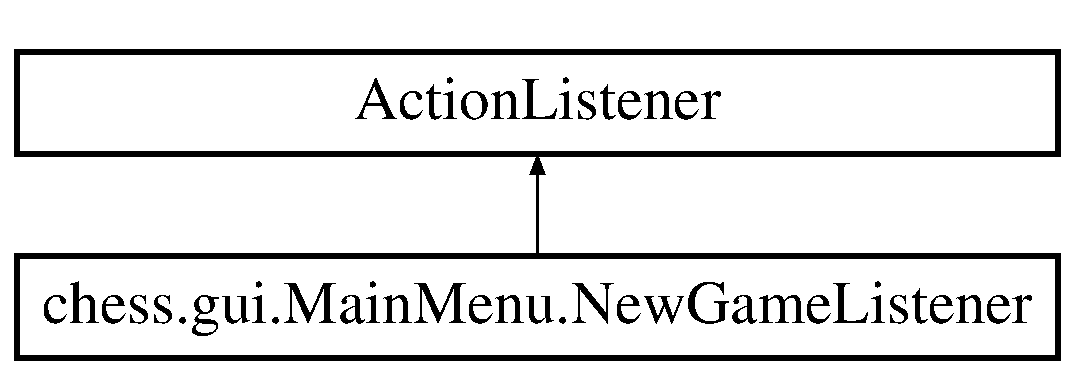
\includegraphics[height=2.000000cm]{classchess_1_1gui_1_1_main_menu_1_1_new_game_listener}
\end{center}
\end{figure}
\subsection*{Public Member Functions}
\begin{DoxyCompactItemize}
\item 
void {\bf action\+Performed} (Action\+Event action\+Event)
\end{DoxyCompactItemize}


\subsection{Member Function Documentation}
\index{chess\+::gui\+::\+Main\+Menu\+::\+New\+Game\+Listener@{chess\+::gui\+::\+Main\+Menu\+::\+New\+Game\+Listener}!action\+Performed@{action\+Performed}}
\index{action\+Performed@{action\+Performed}!chess\+::gui\+::\+Main\+Menu\+::\+New\+Game\+Listener@{chess\+::gui\+::\+Main\+Menu\+::\+New\+Game\+Listener}}
\subsubsection[{action\+Performed}]{\setlength{\rightskip}{0pt plus 5cm}void chess.\+gui.\+Main\+Menu.\+New\+Game\+Listener.\+action\+Performed (
\begin{DoxyParamCaption}
\item[{Action\+Event}]{action\+Event}
\end{DoxyParamCaption}
)}\label{classchess_1_1gui_1_1_main_menu_1_1_new_game_listener_a45dbbb9277dd9362f1d901e6588082bc}


The documentation for this class was generated from the following file\+:\begin{DoxyCompactItemize}
\item 
src/chess/gui/{\bf Main\+Menu.\+java}\end{DoxyCompactItemize}

\section{chess.\+gui.\+New\+Game\+Menu Class Reference}
\label{classchess_1_1gui_1_1_new_game_menu}\index{chess.\+gui.\+New\+Game\+Menu@{chess.\+gui.\+New\+Game\+Menu}}
\subsection*{Public Member Functions}
\begin{DoxyCompactItemize}
\item 
J\+Panel {\bf get\+Pnl\+Upper} ()
\item 
J\+Panel {\bf get\+Pnl\+Lower} ()
\item 
{\bf New\+Game\+Menu} ()
\end{DoxyCompactItemize}


\subsection{Detailed Description}
Created by Fez on 9/17/14. 

\subsection{Constructor \& Destructor Documentation}
\index{chess\+::gui\+::\+New\+Game\+Menu@{chess\+::gui\+::\+New\+Game\+Menu}!New\+Game\+Menu@{New\+Game\+Menu}}
\index{New\+Game\+Menu@{New\+Game\+Menu}!chess\+::gui\+::\+New\+Game\+Menu@{chess\+::gui\+::\+New\+Game\+Menu}}
\subsubsection[{New\+Game\+Menu}]{\setlength{\rightskip}{0pt plus 5cm}chess.\+gui.\+New\+Game\+Menu.\+New\+Game\+Menu (
\begin{DoxyParamCaption}
{}
\end{DoxyParamCaption}
)}\label{classchess_1_1gui_1_1_new_game_menu_a0939daea9ced920068e99b2fdfddcdb8}


\subsection{Member Function Documentation}
\index{chess\+::gui\+::\+New\+Game\+Menu@{chess\+::gui\+::\+New\+Game\+Menu}!get\+Pnl\+Lower@{get\+Pnl\+Lower}}
\index{get\+Pnl\+Lower@{get\+Pnl\+Lower}!chess\+::gui\+::\+New\+Game\+Menu@{chess\+::gui\+::\+New\+Game\+Menu}}
\subsubsection[{get\+Pnl\+Lower}]{\setlength{\rightskip}{0pt plus 5cm}J\+Panel chess.\+gui.\+New\+Game\+Menu.\+get\+Pnl\+Lower (
\begin{DoxyParamCaption}
{}
\end{DoxyParamCaption}
)}\label{classchess_1_1gui_1_1_new_game_menu_addf03e420cadf35d82b6ce29075808c9}
\index{chess\+::gui\+::\+New\+Game\+Menu@{chess\+::gui\+::\+New\+Game\+Menu}!get\+Pnl\+Upper@{get\+Pnl\+Upper}}
\index{get\+Pnl\+Upper@{get\+Pnl\+Upper}!chess\+::gui\+::\+New\+Game\+Menu@{chess\+::gui\+::\+New\+Game\+Menu}}
\subsubsection[{get\+Pnl\+Upper}]{\setlength{\rightskip}{0pt plus 5cm}J\+Panel chess.\+gui.\+New\+Game\+Menu.\+get\+Pnl\+Upper (
\begin{DoxyParamCaption}
{}
\end{DoxyParamCaption}
)}\label{classchess_1_1gui_1_1_new_game_menu_ad301a685ee582147edd2f34f4e3bc087}


The documentation for this class was generated from the following file\+:\begin{DoxyCompactItemize}
\item 
src/chess/gui/{\bf New\+Game\+Menu.\+java}\end{DoxyCompactItemize}

\section{chess.\+pieces.\+Pawn Class Reference}
\label{classchess_1_1pieces_1_1_pawn}\index{chess.\+pieces.\+Pawn@{chess.\+pieces.\+Pawn}}
Inheritance diagram for chess.\+pieces.\+Pawn\+:\begin{figure}[H]
\begin{center}
\leavevmode
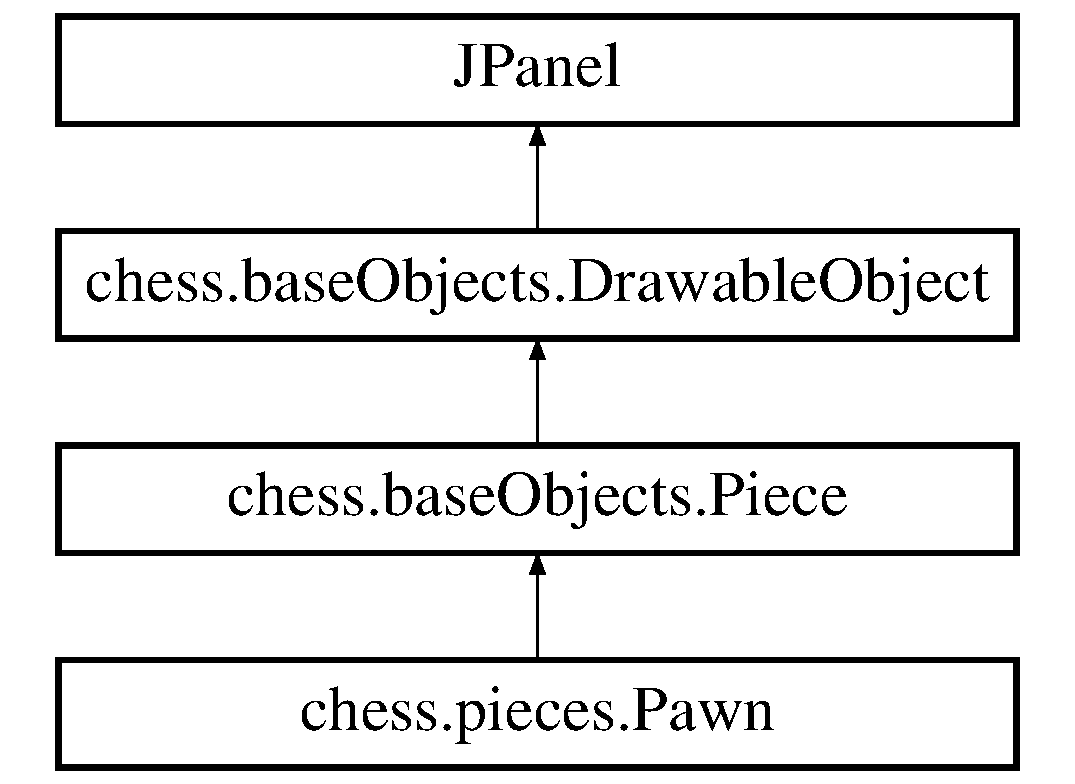
\includegraphics[height=4.000000cm]{classchess_1_1pieces_1_1_pawn}
\end{center}
\end{figure}
\subsection*{Public Member Functions}
\begin{DoxyCompactItemize}
\item 
{\bf Pawn} (String \+\_\+name)
\item 
void {\bf update\+Valid\+Destinations} ({\bf Board} board)
\item 
void {\bf render} (Graphics g)
\end{DoxyCompactItemize}
\subsection*{Additional Inherited Members}


\subsection{Constructor \& Destructor Documentation}
\index{chess\+::pieces\+::\+Pawn@{chess\+::pieces\+::\+Pawn}!Pawn@{Pawn}}
\index{Pawn@{Pawn}!chess\+::pieces\+::\+Pawn@{chess\+::pieces\+::\+Pawn}}
\subsubsection[{Pawn}]{\setlength{\rightskip}{0pt plus 5cm}chess.\+pieces.\+Pawn.\+Pawn (
\begin{DoxyParamCaption}
\item[{String}]{\+\_\+name}
\end{DoxyParamCaption}
)}\label{classchess_1_1pieces_1_1_pawn_a77c289111ed31d98b2821f2827766dd9}


\subsection{Member Function Documentation}
\index{chess\+::pieces\+::\+Pawn@{chess\+::pieces\+::\+Pawn}!render@{render}}
\index{render@{render}!chess\+::pieces\+::\+Pawn@{chess\+::pieces\+::\+Pawn}}
\subsubsection[{render}]{\setlength{\rightskip}{0pt plus 5cm}void chess.\+pieces.\+Pawn.\+render (
\begin{DoxyParamCaption}
\item[{Graphics}]{g}
\end{DoxyParamCaption}
)}\label{classchess_1_1pieces_1_1_pawn_a4a227ec5e5706f298a966b0cf5cf4482}
\index{chess\+::pieces\+::\+Pawn@{chess\+::pieces\+::\+Pawn}!update\+Valid\+Destinations@{update\+Valid\+Destinations}}
\index{update\+Valid\+Destinations@{update\+Valid\+Destinations}!chess\+::pieces\+::\+Pawn@{chess\+::pieces\+::\+Pawn}}
\subsubsection[{update\+Valid\+Destinations}]{\setlength{\rightskip}{0pt plus 5cm}void chess.\+pieces.\+Pawn.\+update\+Valid\+Destinations (
\begin{DoxyParamCaption}
\item[{{\bf Board}}]{board}
\end{DoxyParamCaption}
)}\label{classchess_1_1pieces_1_1_pawn_a9d96562d48c3a1f8d1fbe6cb34e7c74e}


The documentation for this class was generated from the following file\+:\begin{DoxyCompactItemize}
\item 
src/chess/pieces/{\bf Pawn.\+java}\end{DoxyCompactItemize}

\section{chess.\+base\+Objects.\+Piece Class Reference}
\label{classchess_1_1base_objects_1_1_piece}\index{chess.\+base\+Objects.\+Piece@{chess.\+base\+Objects.\+Piece}}
Inheritance diagram for chess.\+base\+Objects.\+Piece\+:\begin{figure}[H]
\begin{center}
\leavevmode
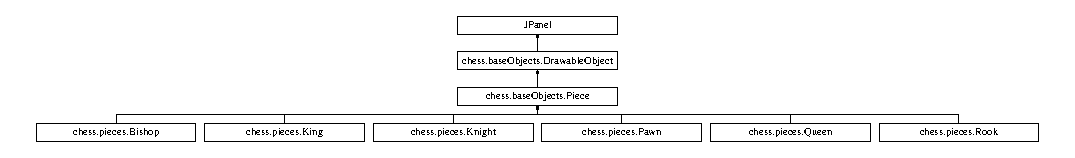
\includegraphics[height=1.681682cm]{classchess_1_1base_objects_1_1_piece}
\end{center}
\end{figure}
\subsection*{Public Member Functions}
\begin{DoxyCompactItemize}
\item 
{\bf Piece} (String d)
\item 
void {\bf set\+Player} ({\bf Player} \+\_\+p)
\item 
{\bf Faction} {\bf get\+Faction} ()
\item 
{\bf Team} {\bf get\+Team} ()
\item 
boolean {\bf can\+Move} ({\bf Square} destination)
\item 
abstract void {\bf update\+Valid\+Destinations} ({\bf Board} board)
\item 
int {\bf get\+Current\+Row} ()
\item 
int {\bf get\+Current\+Column} ()
\item 
boolean {\bf can\+Kill} ({\bf Piece} other)
\end{DoxyCompactItemize}
\subsection*{Static Public Attributes}
\begin{DoxyCompactItemize}
\item 
static final Color {\bf C\+O\+L\+O\+R\+\_\+\+B\+L\+A\+C\+K} = new Color(0x7\+D, 0x5\+A, 0x19)
\item 
static final Color {\bf C\+O\+L\+O\+R\+\_\+\+W\+H\+I\+T\+E} = new Color(0x\+F5, 0x\+D9, 0x\+B5)
\end{DoxyCompactItemize}
\subsection*{Protected Member Functions}
\begin{DoxyCompactItemize}
\item 
void {\bf debug} (String s)
\end{DoxyCompactItemize}
\subsection*{Protected Attributes}
\begin{DoxyCompactItemize}
\item 
Hash\+Set$<$ {\bf Square} $>$ {\bf valid\+Destinations}
\end{DoxyCompactItemize}


\subsection{Constructor \& Destructor Documentation}
\index{chess\+::base\+Objects\+::\+Piece@{chess\+::base\+Objects\+::\+Piece}!Piece@{Piece}}
\index{Piece@{Piece}!chess\+::base\+Objects\+::\+Piece@{chess\+::base\+Objects\+::\+Piece}}
\subsubsection[{Piece}]{\setlength{\rightskip}{0pt plus 5cm}chess.\+base\+Objects.\+Piece.\+Piece (
\begin{DoxyParamCaption}
\item[{String}]{d}
\end{DoxyParamCaption}
)}\label{classchess_1_1base_objects_1_1_piece_a055bdf969f487d1cb02b20e836d40c23}


\subsection{Member Function Documentation}
\index{chess\+::base\+Objects\+::\+Piece@{chess\+::base\+Objects\+::\+Piece}!can\+Kill@{can\+Kill}}
\index{can\+Kill@{can\+Kill}!chess\+::base\+Objects\+::\+Piece@{chess\+::base\+Objects\+::\+Piece}}
\subsubsection[{can\+Kill}]{\setlength{\rightskip}{0pt plus 5cm}boolean chess.\+base\+Objects.\+Piece.\+can\+Kill (
\begin{DoxyParamCaption}
\item[{{\bf Piece}}]{other}
\end{DoxyParamCaption}
)}\label{classchess_1_1base_objects_1_1_piece_a8328f5fd1aca0f4943eec8ad65191305}
\index{chess\+::base\+Objects\+::\+Piece@{chess\+::base\+Objects\+::\+Piece}!can\+Move@{can\+Move}}
\index{can\+Move@{can\+Move}!chess\+::base\+Objects\+::\+Piece@{chess\+::base\+Objects\+::\+Piece}}
\subsubsection[{can\+Move}]{\setlength{\rightskip}{0pt plus 5cm}boolean chess.\+base\+Objects.\+Piece.\+can\+Move (
\begin{DoxyParamCaption}
\item[{{\bf Square}}]{destination}
\end{DoxyParamCaption}
)}\label{classchess_1_1base_objects_1_1_piece_a6fc5d2a29f6733776964bc75117661c5}
\index{chess\+::base\+Objects\+::\+Piece@{chess\+::base\+Objects\+::\+Piece}!debug@{debug}}
\index{debug@{debug}!chess\+::base\+Objects\+::\+Piece@{chess\+::base\+Objects\+::\+Piece}}
\subsubsection[{debug}]{\setlength{\rightskip}{0pt plus 5cm}void chess.\+base\+Objects.\+Piece.\+debug (
\begin{DoxyParamCaption}
\item[{String}]{s}
\end{DoxyParamCaption}
)\hspace{0.3cm}{\ttfamily [protected]}}\label{classchess_1_1base_objects_1_1_piece_a37db685a2fe422798dcdb9fd9316e974}
\index{chess\+::base\+Objects\+::\+Piece@{chess\+::base\+Objects\+::\+Piece}!get\+Current\+Column@{get\+Current\+Column}}
\index{get\+Current\+Column@{get\+Current\+Column}!chess\+::base\+Objects\+::\+Piece@{chess\+::base\+Objects\+::\+Piece}}
\subsubsection[{get\+Current\+Column}]{\setlength{\rightskip}{0pt plus 5cm}int chess.\+base\+Objects.\+Piece.\+get\+Current\+Column (
\begin{DoxyParamCaption}
{}
\end{DoxyParamCaption}
)}\label{classchess_1_1base_objects_1_1_piece_ab44bc5252d49609b433e1e224e4effad}
\index{chess\+::base\+Objects\+::\+Piece@{chess\+::base\+Objects\+::\+Piece}!get\+Current\+Row@{get\+Current\+Row}}
\index{get\+Current\+Row@{get\+Current\+Row}!chess\+::base\+Objects\+::\+Piece@{chess\+::base\+Objects\+::\+Piece}}
\subsubsection[{get\+Current\+Row}]{\setlength{\rightskip}{0pt plus 5cm}int chess.\+base\+Objects.\+Piece.\+get\+Current\+Row (
\begin{DoxyParamCaption}
{}
\end{DoxyParamCaption}
)}\label{classchess_1_1base_objects_1_1_piece_aad2e1a11cfccb3c070df0ae8bdcae96e}
\index{chess\+::base\+Objects\+::\+Piece@{chess\+::base\+Objects\+::\+Piece}!get\+Faction@{get\+Faction}}
\index{get\+Faction@{get\+Faction}!chess\+::base\+Objects\+::\+Piece@{chess\+::base\+Objects\+::\+Piece}}
\subsubsection[{get\+Faction}]{\setlength{\rightskip}{0pt plus 5cm}{\bf Faction} chess.\+base\+Objects.\+Piece.\+get\+Faction (
\begin{DoxyParamCaption}
{}
\end{DoxyParamCaption}
)}\label{classchess_1_1base_objects_1_1_piece_a8a5266ebbe7bd3e6b17091d030685964}
\index{chess\+::base\+Objects\+::\+Piece@{chess\+::base\+Objects\+::\+Piece}!get\+Team@{get\+Team}}
\index{get\+Team@{get\+Team}!chess\+::base\+Objects\+::\+Piece@{chess\+::base\+Objects\+::\+Piece}}
\subsubsection[{get\+Team}]{\setlength{\rightskip}{0pt plus 5cm}{\bf Team} chess.\+base\+Objects.\+Piece.\+get\+Team (
\begin{DoxyParamCaption}
{}
\end{DoxyParamCaption}
)}\label{classchess_1_1base_objects_1_1_piece_a53bd38e2b6fd23bd8e055385f50590ff}
\index{chess\+::base\+Objects\+::\+Piece@{chess\+::base\+Objects\+::\+Piece}!set\+Player@{set\+Player}}
\index{set\+Player@{set\+Player}!chess\+::base\+Objects\+::\+Piece@{chess\+::base\+Objects\+::\+Piece}}
\subsubsection[{set\+Player}]{\setlength{\rightskip}{0pt plus 5cm}void chess.\+base\+Objects.\+Piece.\+set\+Player (
\begin{DoxyParamCaption}
\item[{{\bf Player}}]{\+\_\+p}
\end{DoxyParamCaption}
)}\label{classchess_1_1base_objects_1_1_piece_a592416aa9ea4cec980255c22c33f25e6}
\index{chess\+::base\+Objects\+::\+Piece@{chess\+::base\+Objects\+::\+Piece}!update\+Valid\+Destinations@{update\+Valid\+Destinations}}
\index{update\+Valid\+Destinations@{update\+Valid\+Destinations}!chess\+::base\+Objects\+::\+Piece@{chess\+::base\+Objects\+::\+Piece}}
\subsubsection[{update\+Valid\+Destinations}]{\setlength{\rightskip}{0pt plus 5cm}abstract void chess.\+base\+Objects.\+Piece.\+update\+Valid\+Destinations (
\begin{DoxyParamCaption}
\item[{{\bf Board}}]{board}
\end{DoxyParamCaption}
)\hspace{0.3cm}{\ttfamily [abstract]}}\label{classchess_1_1base_objects_1_1_piece_a70d403304e0965c3910bd3daf50c558c}


\subsection{Member Data Documentation}
\index{chess\+::base\+Objects\+::\+Piece@{chess\+::base\+Objects\+::\+Piece}!C\+O\+L\+O\+R\+\_\+\+B\+L\+A\+C\+K@{C\+O\+L\+O\+R\+\_\+\+B\+L\+A\+C\+K}}
\index{C\+O\+L\+O\+R\+\_\+\+B\+L\+A\+C\+K@{C\+O\+L\+O\+R\+\_\+\+B\+L\+A\+C\+K}!chess\+::base\+Objects\+::\+Piece@{chess\+::base\+Objects\+::\+Piece}}
\subsubsection[{C\+O\+L\+O\+R\+\_\+\+B\+L\+A\+C\+K}]{\setlength{\rightskip}{0pt plus 5cm}final Color chess.\+base\+Objects.\+Piece.\+C\+O\+L\+O\+R\+\_\+\+B\+L\+A\+C\+K = new Color(0x7\+D, 0x5\+A, 0x19)\hspace{0.3cm}{\ttfamily [static]}}\label{classchess_1_1base_objects_1_1_piece_a87b4de4ab8ef5d0650f29fed4842c558}
\index{chess\+::base\+Objects\+::\+Piece@{chess\+::base\+Objects\+::\+Piece}!C\+O\+L\+O\+R\+\_\+\+W\+H\+I\+T\+E@{C\+O\+L\+O\+R\+\_\+\+W\+H\+I\+T\+E}}
\index{C\+O\+L\+O\+R\+\_\+\+W\+H\+I\+T\+E@{C\+O\+L\+O\+R\+\_\+\+W\+H\+I\+T\+E}!chess\+::base\+Objects\+::\+Piece@{chess\+::base\+Objects\+::\+Piece}}
\subsubsection[{C\+O\+L\+O\+R\+\_\+\+W\+H\+I\+T\+E}]{\setlength{\rightskip}{0pt plus 5cm}final Color chess.\+base\+Objects.\+Piece.\+C\+O\+L\+O\+R\+\_\+\+W\+H\+I\+T\+E = new Color(0x\+F5, 0x\+D9, 0x\+B5)\hspace{0.3cm}{\ttfamily [static]}}\label{classchess_1_1base_objects_1_1_piece_a261f183a268678ad026ed6d20c50186a}
\index{chess\+::base\+Objects\+::\+Piece@{chess\+::base\+Objects\+::\+Piece}!valid\+Destinations@{valid\+Destinations}}
\index{valid\+Destinations@{valid\+Destinations}!chess\+::base\+Objects\+::\+Piece@{chess\+::base\+Objects\+::\+Piece}}
\subsubsection[{valid\+Destinations}]{\setlength{\rightskip}{0pt plus 5cm}Hash\+Set$<${\bf Square}$>$ chess.\+base\+Objects.\+Piece.\+valid\+Destinations\hspace{0.3cm}{\ttfamily [protected]}}\label{classchess_1_1base_objects_1_1_piece_a0c9d66088260e46287762e973669ef3b}


The documentation for this class was generated from the following file\+:\begin{DoxyCompactItemize}
\item 
src/chess/base\+Objects/{\bf Piece.\+java}\end{DoxyCompactItemize}

\section{chess.\+base\+Objects.\+Player Class Reference}
\label{classchess_1_1base_objects_1_1_player}\index{chess.\+base\+Objects.\+Player@{chess.\+base\+Objects.\+Player}}
\subsection*{Public Member Functions}
\begin{DoxyCompactItemize}
\item 
{\bf Player} ({\bf Team} \+\_\+t, {\bf Faction} \+\_\+f)
\item 
void {\bf move} ({\bf Piece} p, {\bf Square} destination)
\item 
{\bf Faction} {\bf get\+Faction} ()
\item 
{\bf Team} {\bf get\+Team} ()
\end{DoxyCompactItemize}


\subsection{Constructor \& Destructor Documentation}
\index{chess\+::base\+Objects\+::\+Player@{chess\+::base\+Objects\+::\+Player}!Player@{Player}}
\index{Player@{Player}!chess\+::base\+Objects\+::\+Player@{chess\+::base\+Objects\+::\+Player}}
\subsubsection[{Player}]{\setlength{\rightskip}{0pt plus 5cm}chess.\+base\+Objects.\+Player.\+Player (
\begin{DoxyParamCaption}
\item[{{\bf Team}}]{\+\_\+t, }
\item[{{\bf Faction}}]{\+\_\+f}
\end{DoxyParamCaption}
)}\label{classchess_1_1base_objects_1_1_player_a4eff607d6bbfc3fe8114e9db548b5997}


\subsection{Member Function Documentation}
\index{chess\+::base\+Objects\+::\+Player@{chess\+::base\+Objects\+::\+Player}!get\+Faction@{get\+Faction}}
\index{get\+Faction@{get\+Faction}!chess\+::base\+Objects\+::\+Player@{chess\+::base\+Objects\+::\+Player}}
\subsubsection[{get\+Faction}]{\setlength{\rightskip}{0pt plus 5cm}{\bf Faction} chess.\+base\+Objects.\+Player.\+get\+Faction (
\begin{DoxyParamCaption}
{}
\end{DoxyParamCaption}
)}\label{classchess_1_1base_objects_1_1_player_a33bd3243305b45b72b1c2b29b639cc8e}
\index{chess\+::base\+Objects\+::\+Player@{chess\+::base\+Objects\+::\+Player}!get\+Team@{get\+Team}}
\index{get\+Team@{get\+Team}!chess\+::base\+Objects\+::\+Player@{chess\+::base\+Objects\+::\+Player}}
\subsubsection[{get\+Team}]{\setlength{\rightskip}{0pt plus 5cm}{\bf Team} chess.\+base\+Objects.\+Player.\+get\+Team (
\begin{DoxyParamCaption}
{}
\end{DoxyParamCaption}
)}\label{classchess_1_1base_objects_1_1_player_a65cfcd43bb39f65d83a847d55ab976a0}
\index{chess\+::base\+Objects\+::\+Player@{chess\+::base\+Objects\+::\+Player}!move@{move}}
\index{move@{move}!chess\+::base\+Objects\+::\+Player@{chess\+::base\+Objects\+::\+Player}}
\subsubsection[{move}]{\setlength{\rightskip}{0pt plus 5cm}void chess.\+base\+Objects.\+Player.\+move (
\begin{DoxyParamCaption}
\item[{{\bf Piece}}]{p, }
\item[{{\bf Square}}]{destination}
\end{DoxyParamCaption}
)}\label{classchess_1_1base_objects_1_1_player_af6bfb69753a267e2da7a2d48c361d1fc}


The documentation for this class was generated from the following file\+:\begin{DoxyCompactItemize}
\item 
src/chess/base\+Objects/{\bf Player.\+java}\end{DoxyCompactItemize}

\section{chess.\+pieces.\+Queen Class Reference}
\label{classchess_1_1pieces_1_1_queen}\index{chess.\+pieces.\+Queen@{chess.\+pieces.\+Queen}}
Inheritance diagram for chess.\+pieces.\+Queen\+:\begin{figure}[H]
\begin{center}
\leavevmode
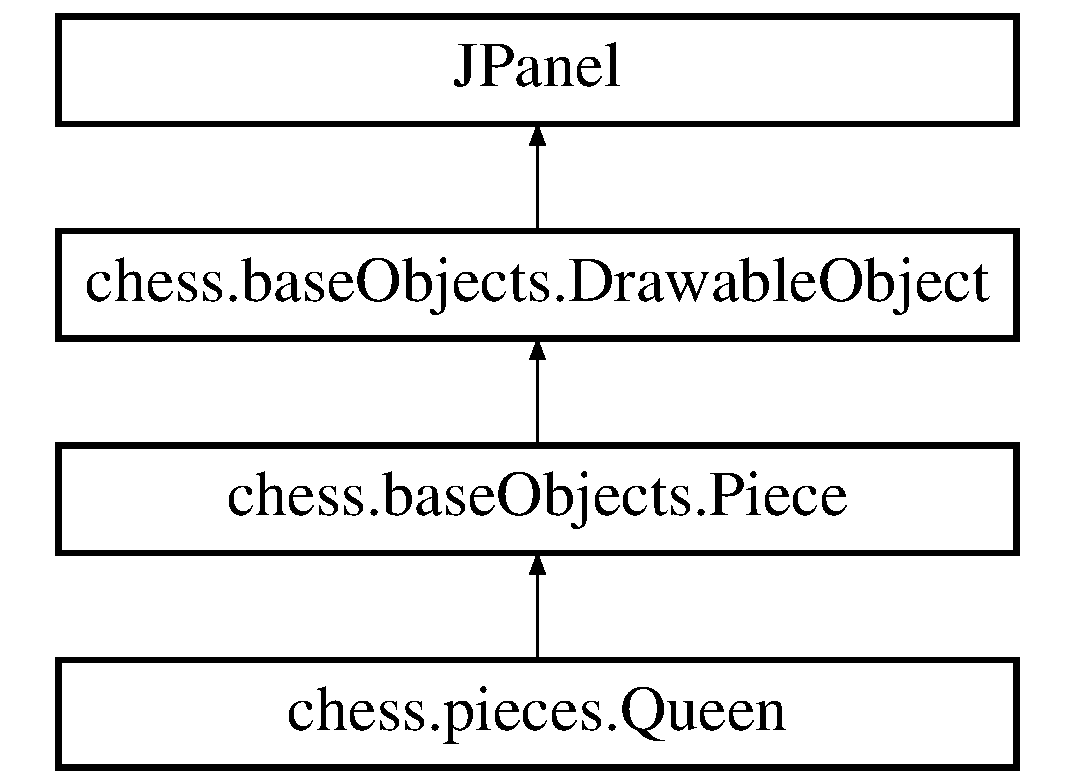
\includegraphics[height=4.000000cm]{classchess_1_1pieces_1_1_queen}
\end{center}
\end{figure}
\subsection*{Public Member Functions}
\begin{DoxyCompactItemize}
\item 
{\bf Queen} (String \+\_\+name)
\item 
void {\bf update\+Valid\+Destinations} ({\bf Board} board)
\item 
void {\bf render} (Graphics g)
\end{DoxyCompactItemize}
\subsection*{Additional Inherited Members}


\subsection{Constructor \& Destructor Documentation}
\index{chess\+::pieces\+::\+Queen@{chess\+::pieces\+::\+Queen}!Queen@{Queen}}
\index{Queen@{Queen}!chess\+::pieces\+::\+Queen@{chess\+::pieces\+::\+Queen}}
\subsubsection[{Queen}]{\setlength{\rightskip}{0pt plus 5cm}chess.\+pieces.\+Queen.\+Queen (
\begin{DoxyParamCaption}
\item[{String}]{\+\_\+name}
\end{DoxyParamCaption}
)}\label{classchess_1_1pieces_1_1_queen_ad1ec0c9708098454d0f98933a6a32c9e}


\subsection{Member Function Documentation}
\index{chess\+::pieces\+::\+Queen@{chess\+::pieces\+::\+Queen}!render@{render}}
\index{render@{render}!chess\+::pieces\+::\+Queen@{chess\+::pieces\+::\+Queen}}
\subsubsection[{render}]{\setlength{\rightskip}{0pt plus 5cm}void chess.\+pieces.\+Queen.\+render (
\begin{DoxyParamCaption}
\item[{Graphics}]{g}
\end{DoxyParamCaption}
)}\label{classchess_1_1pieces_1_1_queen_a8f763550f3e7f3f1f3932040c4475bbf}
\index{chess\+::pieces\+::\+Queen@{chess\+::pieces\+::\+Queen}!update\+Valid\+Destinations@{update\+Valid\+Destinations}}
\index{update\+Valid\+Destinations@{update\+Valid\+Destinations}!chess\+::pieces\+::\+Queen@{chess\+::pieces\+::\+Queen}}
\subsubsection[{update\+Valid\+Destinations}]{\setlength{\rightskip}{0pt plus 5cm}void chess.\+pieces.\+Queen.\+update\+Valid\+Destinations (
\begin{DoxyParamCaption}
\item[{{\bf Board}}]{board}
\end{DoxyParamCaption}
)}\label{classchess_1_1pieces_1_1_queen_acc28cb67c6a69256427f97c97f4a5f89}


The documentation for this class was generated from the following file\+:\begin{DoxyCompactItemize}
\item 
src/chess/pieces/{\bf Queen.\+java}\end{DoxyCompactItemize}

\section{chess.\+gui.\+Main\+Menu.\+Quit\+Listener Class Reference}
\label{classchess_1_1gui_1_1_main_menu_1_1_quit_listener}\index{chess.\+gui.\+Main\+Menu.\+Quit\+Listener@{chess.\+gui.\+Main\+Menu.\+Quit\+Listener}}
Inheritance diagram for chess.\+gui.\+Main\+Menu.\+Quit\+Listener\+:\begin{figure}[H]
\begin{center}
\leavevmode
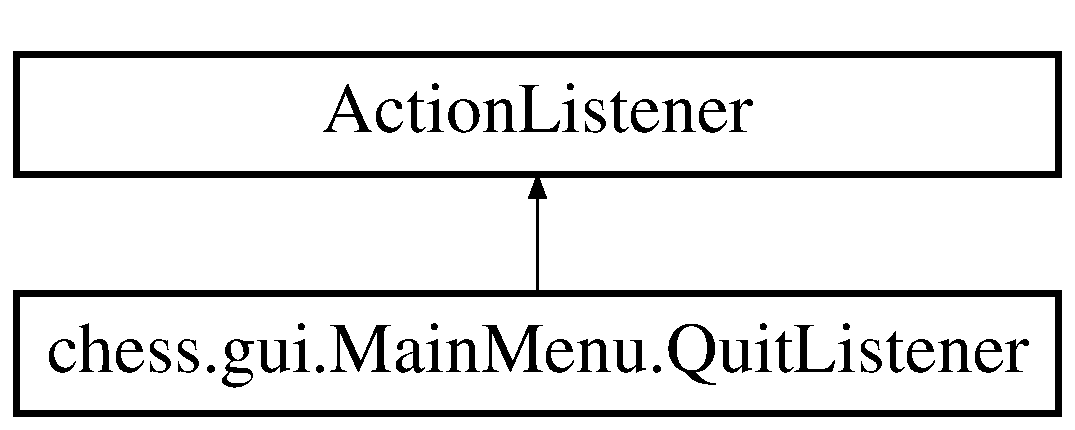
\includegraphics[height=2.000000cm]{classchess_1_1gui_1_1_main_menu_1_1_quit_listener}
\end{center}
\end{figure}
\subsection*{Public Member Functions}
\begin{DoxyCompactItemize}
\item 
void {\bf action\+Performed} (Action\+Event action\+Event)
\end{DoxyCompactItemize}


\subsection{Member Function Documentation}
\index{chess\+::gui\+::\+Main\+Menu\+::\+Quit\+Listener@{chess\+::gui\+::\+Main\+Menu\+::\+Quit\+Listener}!action\+Performed@{action\+Performed}}
\index{action\+Performed@{action\+Performed}!chess\+::gui\+::\+Main\+Menu\+::\+Quit\+Listener@{chess\+::gui\+::\+Main\+Menu\+::\+Quit\+Listener}}
\subsubsection[{action\+Performed}]{\setlength{\rightskip}{0pt plus 5cm}void chess.\+gui.\+Main\+Menu.\+Quit\+Listener.\+action\+Performed (
\begin{DoxyParamCaption}
\item[{Action\+Event}]{action\+Event}
\end{DoxyParamCaption}
)}\label{classchess_1_1gui_1_1_main_menu_1_1_quit_listener_abdc1e8a89a28a5d648ca5954bc1b49f6}


The documentation for this class was generated from the following file\+:\begin{DoxyCompactItemize}
\item 
src/chess/gui/{\bf Main\+Menu.\+java}\end{DoxyCompactItemize}

\section{chess.\+pieces.\+Rook Class Reference}
\label{classchess_1_1pieces_1_1_rook}\index{chess.\+pieces.\+Rook@{chess.\+pieces.\+Rook}}
Inheritance diagram for chess.\+pieces.\+Rook\+:\begin{figure}[H]
\begin{center}
\leavevmode
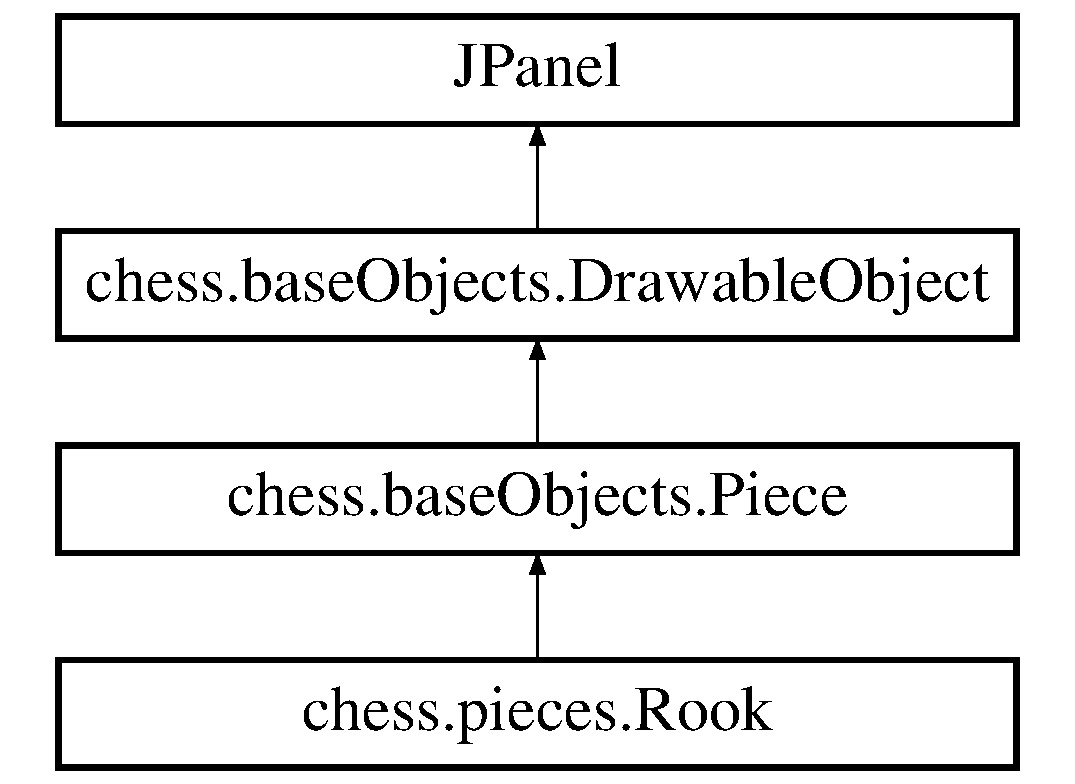
\includegraphics[height=4.000000cm]{classchess_1_1pieces_1_1_rook}
\end{center}
\end{figure}
\subsection*{Public Member Functions}
\begin{DoxyCompactItemize}
\item 
{\bf Rook} (String \+\_\+name)
\item 
void {\bf update\+Valid\+Destinations} ({\bf Board} board)
\item 
void {\bf render} (Graphics g)
\end{DoxyCompactItemize}
\subsection*{Additional Inherited Members}


\subsection{Constructor \& Destructor Documentation}
\index{chess\+::pieces\+::\+Rook@{chess\+::pieces\+::\+Rook}!Rook@{Rook}}
\index{Rook@{Rook}!chess\+::pieces\+::\+Rook@{chess\+::pieces\+::\+Rook}}
\subsubsection[{Rook}]{\setlength{\rightskip}{0pt plus 5cm}chess.\+pieces.\+Rook.\+Rook (
\begin{DoxyParamCaption}
\item[{String}]{\+\_\+name}
\end{DoxyParamCaption}
)}\label{classchess_1_1pieces_1_1_rook_a7fbb81f604f68d1076f151983a566451}


\subsection{Member Function Documentation}
\index{chess\+::pieces\+::\+Rook@{chess\+::pieces\+::\+Rook}!render@{render}}
\index{render@{render}!chess\+::pieces\+::\+Rook@{chess\+::pieces\+::\+Rook}}
\subsubsection[{render}]{\setlength{\rightskip}{0pt plus 5cm}void chess.\+pieces.\+Rook.\+render (
\begin{DoxyParamCaption}
\item[{Graphics}]{g}
\end{DoxyParamCaption}
)}\label{classchess_1_1pieces_1_1_rook_ada777a38ef1e638fcf3f61bc06a71cf5}
\index{chess\+::pieces\+::\+Rook@{chess\+::pieces\+::\+Rook}!update\+Valid\+Destinations@{update\+Valid\+Destinations}}
\index{update\+Valid\+Destinations@{update\+Valid\+Destinations}!chess\+::pieces\+::\+Rook@{chess\+::pieces\+::\+Rook}}
\subsubsection[{update\+Valid\+Destinations}]{\setlength{\rightskip}{0pt plus 5cm}void chess.\+pieces.\+Rook.\+update\+Valid\+Destinations (
\begin{DoxyParamCaption}
\item[{{\bf Board}}]{board}
\end{DoxyParamCaption}
)}\label{classchess_1_1pieces_1_1_rook_a6ad309a0010e51b79f894501bc054559}


The documentation for this class was generated from the following file\+:\begin{DoxyCompactItemize}
\item 
src/chess/pieces/{\bf Rook.\+java}\end{DoxyCompactItemize}

\section{chess.\+master.\+Runner Class Reference}
\label{classchess_1_1master_1_1_runner}\index{chess.\+master.\+Runner@{chess.\+master.\+Runner}}
\subsection*{Static Public Member Functions}
\begin{DoxyCompactItemize}
\item 
static void {\bf main} (String[$\,$] args)
\end{DoxyCompactItemize}


\subsection{Member Function Documentation}
\index{chess\+::master\+::\+Runner@{chess\+::master\+::\+Runner}!main@{main}}
\index{main@{main}!chess\+::master\+::\+Runner@{chess\+::master\+::\+Runner}}
\subsubsection[{main}]{\setlength{\rightskip}{0pt plus 5cm}static void chess.\+master.\+Runner.\+main (
\begin{DoxyParamCaption}
\item[{String[$\,$]}]{args}
\end{DoxyParamCaption}
)\hspace{0.3cm}{\ttfamily [static]}}\label{classchess_1_1master_1_1_runner_aa765e23ac2ff2dde2f912a844b818e65}


The documentation for this class was generated from the following file\+:\begin{DoxyCompactItemize}
\item 
src/chess/master/{\bf Runner.\+java}\end{DoxyCompactItemize}

\section{chess.\+gui.\+Main\+Menu.\+Settings\+Listener Class Reference}
\label{classchess_1_1gui_1_1_main_menu_1_1_settings_listener}\index{chess.\+gui.\+Main\+Menu.\+Settings\+Listener@{chess.\+gui.\+Main\+Menu.\+Settings\+Listener}}
Inheritance diagram for chess.\+gui.\+Main\+Menu.\+Settings\+Listener\+:\begin{figure}[H]
\begin{center}
\leavevmode
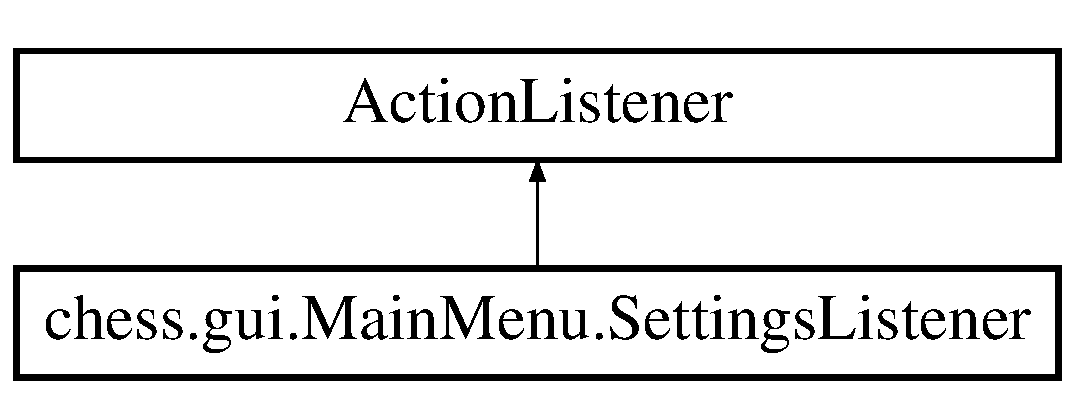
\includegraphics[height=2.000000cm]{classchess_1_1gui_1_1_main_menu_1_1_settings_listener}
\end{center}
\end{figure}
\subsection*{Public Member Functions}
\begin{DoxyCompactItemize}
\item 
void {\bf action\+Performed} (Action\+Event action\+Event)
\end{DoxyCompactItemize}


\subsection{Member Function Documentation}
\index{chess\+::gui\+::\+Main\+Menu\+::\+Settings\+Listener@{chess\+::gui\+::\+Main\+Menu\+::\+Settings\+Listener}!action\+Performed@{action\+Performed}}
\index{action\+Performed@{action\+Performed}!chess\+::gui\+::\+Main\+Menu\+::\+Settings\+Listener@{chess\+::gui\+::\+Main\+Menu\+::\+Settings\+Listener}}
\subsubsection[{action\+Performed}]{\setlength{\rightskip}{0pt plus 5cm}void chess.\+gui.\+Main\+Menu.\+Settings\+Listener.\+action\+Performed (
\begin{DoxyParamCaption}
\item[{Action\+Event}]{action\+Event}
\end{DoxyParamCaption}
)}\label{classchess_1_1gui_1_1_main_menu_1_1_settings_listener_a51ccc652e93c6643003b793c23e0c16f}


The documentation for this class was generated from the following file\+:\begin{DoxyCompactItemize}
\item 
src/chess/gui/{\bf Main\+Menu.\+java}\end{DoxyCompactItemize}

\section{chess.\+base\+Objects.\+Square Class Reference}
\label{classchess_1_1base_objects_1_1_square}\index{chess.\+base\+Objects.\+Square@{chess.\+base\+Objects.\+Square}}
Inheritance diagram for chess.\+base\+Objects.\+Square\+:\begin{figure}[H]
\begin{center}
\leavevmode
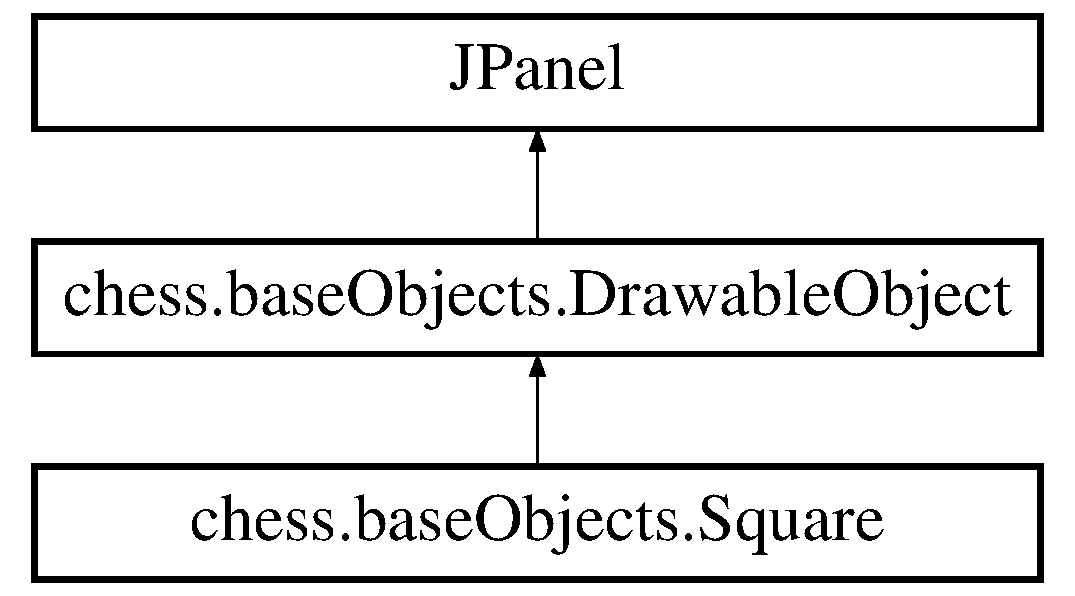
\includegraphics[height=3.000000cm]{classchess_1_1base_objects_1_1_square}
\end{center}
\end{figure}
\subsection*{Classes}
\begin{DoxyCompactItemize}
\item 
class {\bfseries Coordinate}
\end{DoxyCompactItemize}
\subsection*{Public Member Functions}
\begin{DoxyCompactItemize}
\item 
boolean {\bf has\+Piece} ()
\item 
{\bf Piece} {\bf get\+Piece} ()
\item 
boolean {\bf set\+Piece} ({\bf Piece} p)
\item 
boolean {\bf get\+Color} ()
\item 
{\bf Square} (int \+\_\+col, int \+\_\+row, boolean \+\_\+color)
\item 
void {\bf render} (Graphics g)
\item 
int {\bf get\+Row} ()
\item 
void {\bf set\+Row} (int row)
\item 
int {\bf get\+Column} ()
\item 
void {\bf set\+Column} (int column)
\end{DoxyCompactItemize}
\subsection*{Static Public Member Functions}
\begin{DoxyCompactItemize}
\item 
static void {\bf set\+Width} (int w)
\end{DoxyCompactItemize}


\subsection{Constructor \& Destructor Documentation}
\index{chess\+::base\+Objects\+::\+Square@{chess\+::base\+Objects\+::\+Square}!Square@{Square}}
\index{Square@{Square}!chess\+::base\+Objects\+::\+Square@{chess\+::base\+Objects\+::\+Square}}
\subsubsection[{Square}]{\setlength{\rightskip}{0pt plus 5cm}chess.\+base\+Objects.\+Square.\+Square (
\begin{DoxyParamCaption}
\item[{int}]{\+\_\+col, }
\item[{int}]{\+\_\+row, }
\item[{boolean}]{\+\_\+color}
\end{DoxyParamCaption}
)}\label{classchess_1_1base_objects_1_1_square_aeb8f7d5c5e75d69e6a70c6e5a025974f}


\subsection{Member Function Documentation}
\index{chess\+::base\+Objects\+::\+Square@{chess\+::base\+Objects\+::\+Square}!get\+Color@{get\+Color}}
\index{get\+Color@{get\+Color}!chess\+::base\+Objects\+::\+Square@{chess\+::base\+Objects\+::\+Square}}
\subsubsection[{get\+Color}]{\setlength{\rightskip}{0pt plus 5cm}boolean chess.\+base\+Objects.\+Square.\+get\+Color (
\begin{DoxyParamCaption}
{}
\end{DoxyParamCaption}
)}\label{classchess_1_1base_objects_1_1_square_a2f60d00875ca4e2273507d471bd6b745}
\index{chess\+::base\+Objects\+::\+Square@{chess\+::base\+Objects\+::\+Square}!get\+Column@{get\+Column}}
\index{get\+Column@{get\+Column}!chess\+::base\+Objects\+::\+Square@{chess\+::base\+Objects\+::\+Square}}
\subsubsection[{get\+Column}]{\setlength{\rightskip}{0pt plus 5cm}int chess.\+base\+Objects.\+Square.\+get\+Column (
\begin{DoxyParamCaption}
{}
\end{DoxyParamCaption}
)}\label{classchess_1_1base_objects_1_1_square_a75db56550fe497a56bb8922bf03a2cd5}
\index{chess\+::base\+Objects\+::\+Square@{chess\+::base\+Objects\+::\+Square}!get\+Piece@{get\+Piece}}
\index{get\+Piece@{get\+Piece}!chess\+::base\+Objects\+::\+Square@{chess\+::base\+Objects\+::\+Square}}
\subsubsection[{get\+Piece}]{\setlength{\rightskip}{0pt plus 5cm}{\bf Piece} chess.\+base\+Objects.\+Square.\+get\+Piece (
\begin{DoxyParamCaption}
{}
\end{DoxyParamCaption}
)}\label{classchess_1_1base_objects_1_1_square_a6c21e2147a6db464905cdf7beeea1ce4}
\index{chess\+::base\+Objects\+::\+Square@{chess\+::base\+Objects\+::\+Square}!get\+Row@{get\+Row}}
\index{get\+Row@{get\+Row}!chess\+::base\+Objects\+::\+Square@{chess\+::base\+Objects\+::\+Square}}
\subsubsection[{get\+Row}]{\setlength{\rightskip}{0pt plus 5cm}int chess.\+base\+Objects.\+Square.\+get\+Row (
\begin{DoxyParamCaption}
{}
\end{DoxyParamCaption}
)}\label{classchess_1_1base_objects_1_1_square_ae9f625154da651047c630f0825df1fc6}
\index{chess\+::base\+Objects\+::\+Square@{chess\+::base\+Objects\+::\+Square}!has\+Piece@{has\+Piece}}
\index{has\+Piece@{has\+Piece}!chess\+::base\+Objects\+::\+Square@{chess\+::base\+Objects\+::\+Square}}
\subsubsection[{has\+Piece}]{\setlength{\rightskip}{0pt plus 5cm}boolean chess.\+base\+Objects.\+Square.\+has\+Piece (
\begin{DoxyParamCaption}
{}
\end{DoxyParamCaption}
)}\label{classchess_1_1base_objects_1_1_square_a182f6c68d67b9e0f1e4dc7a21007cc0e}
\index{chess\+::base\+Objects\+::\+Square@{chess\+::base\+Objects\+::\+Square}!render@{render}}
\index{render@{render}!chess\+::base\+Objects\+::\+Square@{chess\+::base\+Objects\+::\+Square}}
\subsubsection[{render}]{\setlength{\rightskip}{0pt plus 5cm}void chess.\+base\+Objects.\+Square.\+render (
\begin{DoxyParamCaption}
\item[{Graphics}]{g}
\end{DoxyParamCaption}
)}\label{classchess_1_1base_objects_1_1_square_a674f4fbb1a82c76fd02d8ec5b8007d0d}
\index{chess\+::base\+Objects\+::\+Square@{chess\+::base\+Objects\+::\+Square}!set\+Column@{set\+Column}}
\index{set\+Column@{set\+Column}!chess\+::base\+Objects\+::\+Square@{chess\+::base\+Objects\+::\+Square}}
\subsubsection[{set\+Column}]{\setlength{\rightskip}{0pt plus 5cm}void chess.\+base\+Objects.\+Square.\+set\+Column (
\begin{DoxyParamCaption}
\item[{int}]{column}
\end{DoxyParamCaption}
)}\label{classchess_1_1base_objects_1_1_square_a8d6bd3a22cf16e3c8289b97879f9be32}
\index{chess\+::base\+Objects\+::\+Square@{chess\+::base\+Objects\+::\+Square}!set\+Piece@{set\+Piece}}
\index{set\+Piece@{set\+Piece}!chess\+::base\+Objects\+::\+Square@{chess\+::base\+Objects\+::\+Square}}
\subsubsection[{set\+Piece}]{\setlength{\rightskip}{0pt plus 5cm}boolean chess.\+base\+Objects.\+Square.\+set\+Piece (
\begin{DoxyParamCaption}
\item[{{\bf Piece}}]{p}
\end{DoxyParamCaption}
)}\label{classchess_1_1base_objects_1_1_square_a75eb07f19bc053e9240afd0bb02160dd}
\index{chess\+::base\+Objects\+::\+Square@{chess\+::base\+Objects\+::\+Square}!set\+Row@{set\+Row}}
\index{set\+Row@{set\+Row}!chess\+::base\+Objects\+::\+Square@{chess\+::base\+Objects\+::\+Square}}
\subsubsection[{set\+Row}]{\setlength{\rightskip}{0pt plus 5cm}void chess.\+base\+Objects.\+Square.\+set\+Row (
\begin{DoxyParamCaption}
\item[{int}]{row}
\end{DoxyParamCaption}
)}\label{classchess_1_1base_objects_1_1_square_aa24354faf86a38d21d22b3aad6cdc182}
\index{chess\+::base\+Objects\+::\+Square@{chess\+::base\+Objects\+::\+Square}!set\+Width@{set\+Width}}
\index{set\+Width@{set\+Width}!chess\+::base\+Objects\+::\+Square@{chess\+::base\+Objects\+::\+Square}}
\subsubsection[{set\+Width}]{\setlength{\rightskip}{0pt plus 5cm}static void chess.\+base\+Objects.\+Square.\+set\+Width (
\begin{DoxyParamCaption}
\item[{int}]{w}
\end{DoxyParamCaption}
)\hspace{0.3cm}{\ttfamily [static]}}\label{classchess_1_1base_objects_1_1_square_a8f9bca8b9e4c75f7dcc0e7bd1d418831}


The documentation for this class was generated from the following file\+:\begin{DoxyCompactItemize}
\item 
src/chess/base\+Objects/{\bf Square.\+java}\end{DoxyCompactItemize}

\section{chess.\+base\+Objects.\+Team Class Reference}
\label{classchess_1_1base_objects_1_1_team}\index{chess.\+base\+Objects.\+Team@{chess.\+base\+Objects.\+Team}}
\subsection*{Public Member Functions}
\begin{DoxyCompactItemize}
\item 
{\bf Team} (int num\+Players, {\bf Faction}[$\,$] \+\_\+factions)
\item 
{\bf Player} {\bf get\+Player\+By\+Number} (int i)
\end{DoxyCompactItemize}


\subsection{Constructor \& Destructor Documentation}
\index{chess\+::base\+Objects\+::\+Team@{chess\+::base\+Objects\+::\+Team}!Team@{Team}}
\index{Team@{Team}!chess\+::base\+Objects\+::\+Team@{chess\+::base\+Objects\+::\+Team}}
\subsubsection[{Team}]{\setlength{\rightskip}{0pt plus 5cm}chess.\+base\+Objects.\+Team.\+Team (
\begin{DoxyParamCaption}
\item[{int}]{num\+Players, }
\item[{{\bf Faction}[$\,$]}]{\+\_\+factions}
\end{DoxyParamCaption}
)}\label{classchess_1_1base_objects_1_1_team_a10e1a2bec84aef82feffdf878aed2b5f}


\subsection{Member Function Documentation}
\index{chess\+::base\+Objects\+::\+Team@{chess\+::base\+Objects\+::\+Team}!get\+Player\+By\+Number@{get\+Player\+By\+Number}}
\index{get\+Player\+By\+Number@{get\+Player\+By\+Number}!chess\+::base\+Objects\+::\+Team@{chess\+::base\+Objects\+::\+Team}}
\subsubsection[{get\+Player\+By\+Number}]{\setlength{\rightskip}{0pt plus 5cm}{\bf Player} chess.\+base\+Objects.\+Team.\+get\+Player\+By\+Number (
\begin{DoxyParamCaption}
\item[{int}]{i}
\end{DoxyParamCaption}
)}\label{classchess_1_1base_objects_1_1_team_abe20fa9fc9d57cac59b2ab3f3f5b9a4a}


The documentation for this class was generated from the following file\+:\begin{DoxyCompactItemize}
\item 
src/chess/base\+Objects/{\bf Team.\+java}\end{DoxyCompactItemize}

\section{chess.\+base\+Objects.\+Turn Class Reference}
\label{classchess_1_1base_objects_1_1_turn}\index{chess.\+base\+Objects.\+Turn@{chess.\+base\+Objects.\+Turn}}
\subsection*{Public Member Functions}
\begin{DoxyCompactItemize}
\item 
{\bf Player} {\bf get\+Active\+Player} ()
\end{DoxyCompactItemize}


\subsection{Member Function Documentation}
\index{chess\+::base\+Objects\+::\+Turn@{chess\+::base\+Objects\+::\+Turn}!get\+Active\+Player@{get\+Active\+Player}}
\index{get\+Active\+Player@{get\+Active\+Player}!chess\+::base\+Objects\+::\+Turn@{chess\+::base\+Objects\+::\+Turn}}
\subsubsection[{get\+Active\+Player}]{\setlength{\rightskip}{0pt plus 5cm}{\bf Player} chess.\+base\+Objects.\+Turn.\+get\+Active\+Player (
\begin{DoxyParamCaption}
{}
\end{DoxyParamCaption}
)}\label{classchess_1_1base_objects_1_1_turn_a8bf72a260ec96fe6ddf6c13f5572edcb}


The documentation for this class was generated from the following file\+:\begin{DoxyCompactItemize}
\item 
src/chess/base\+Objects/{\bf Turn.\+java}\end{DoxyCompactItemize}

\section{chess.\+general.\+Utilities Class Reference}
\label{classchess_1_1general_1_1_utilities}\index{chess.\+general.\+Utilities@{chess.\+general.\+Utilities}}
\subsection*{Static Public Member Functions}
\begin{DoxyCompactItemize}
\item 
static$<$ T $>$ Vector$<$ T $>$ {\bf intersect} (Vector$<$ T $>$ a, Vector$<$ T $>$ b)
\item 
static$<$ T $>$ Set$<$ T $>$ {\bf intersect} (Set$<$ T $>$ a, Set$<$ T $>$ b)
\item 
static J\+Button {\bf button\+Factory} (String name, String action, Font f)
\end{DoxyCompactItemize}


\subsection{Detailed Description}
Created by Fez on 9/14/14. 

\subsection{Member Function Documentation}
\index{chess\+::general\+::\+Utilities@{chess\+::general\+::\+Utilities}!button\+Factory@{button\+Factory}}
\index{button\+Factory@{button\+Factory}!chess\+::general\+::\+Utilities@{chess\+::general\+::\+Utilities}}
\subsubsection[{button\+Factory}]{\setlength{\rightskip}{0pt plus 5cm}static J\+Button chess.\+general.\+Utilities.\+button\+Factory (
\begin{DoxyParamCaption}
\item[{String}]{name, }
\item[{String}]{action, }
\item[{Font}]{f}
\end{DoxyParamCaption}
)\hspace{0.3cm}{\ttfamily [static]}}\label{classchess_1_1general_1_1_utilities_a49ccb0fbe6cd227d5c0d51f57a040abc}
\index{chess\+::general\+::\+Utilities@{chess\+::general\+::\+Utilities}!intersect@{intersect}}
\index{intersect@{intersect}!chess\+::general\+::\+Utilities@{chess\+::general\+::\+Utilities}}
\subsubsection[{intersect}]{\setlength{\rightskip}{0pt plus 5cm}static $<$T$>$ Vector$<$T$>$ chess.\+general.\+Utilities.\+intersect (
\begin{DoxyParamCaption}
\item[{Vector$<$ T $>$}]{a, }
\item[{Vector$<$ T $>$}]{b}
\end{DoxyParamCaption}
)\hspace{0.3cm}{\ttfamily [static]}}\label{classchess_1_1general_1_1_utilities_a50b2f8ecc8fcffe554f8df31f458bbff}
\index{chess\+::general\+::\+Utilities@{chess\+::general\+::\+Utilities}!intersect@{intersect}}
\index{intersect@{intersect}!chess\+::general\+::\+Utilities@{chess\+::general\+::\+Utilities}}
\subsubsection[{intersect}]{\setlength{\rightskip}{0pt plus 5cm}static $<$T$>$ Set$<$T$>$ chess.\+general.\+Utilities.\+intersect (
\begin{DoxyParamCaption}
\item[{Set$<$ T $>$}]{a, }
\item[{Set$<$ T $>$}]{b}
\end{DoxyParamCaption}
)\hspace{0.3cm}{\ttfamily [static]}}\label{classchess_1_1general_1_1_utilities_a56abbf77d5e9b3e4a38f23693a553f42}


The documentation for this class was generated from the following file\+:\begin{DoxyCompactItemize}
\item 
src/chess/general/{\bf Utilities.\+java}\end{DoxyCompactItemize}

\chapter{File Documentation}
\section{src/chess/base\+Objects/\+Board.java File Reference}
\label{_board_8java}\index{src/chess/base\+Objects/\+Board.\+java@{src/chess/base\+Objects/\+Board.\+java}}
\subsection*{Classes}
\begin{DoxyCompactItemize}
\item 
class {\bf chess.\+base\+Objects.\+Board}
\item 
class {\bf chess.\+base\+Objects.\+Board.\+Chess\+Board\+Cell\+Renderer}
\end{DoxyCompactItemize}
\subsection*{Packages}
\begin{DoxyCompactItemize}
\item 
package {\bf chess.\+base\+Objects}
\end{DoxyCompactItemize}

\section{src/chess/base\+Objects/\+Drawable\+Object.java File Reference}
\label{_drawable_object_8java}\index{src/chess/base\+Objects/\+Drawable\+Object.\+java@{src/chess/base\+Objects/\+Drawable\+Object.\+java}}
\subsection*{Classes}
\begin{DoxyCompactItemize}
\item 
class {\bf chess.\+base\+Objects.\+Drawable\+Object}
\end{DoxyCompactItemize}
\subsection*{Packages}
\begin{DoxyCompactItemize}
\item 
package {\bf chess.\+base\+Objects}
\end{DoxyCompactItemize}

\section{src/chess/base\+Objects/\+Event.java File Reference}
\label{_event_8java}\index{src/chess/base\+Objects/\+Event.\+java@{src/chess/base\+Objects/\+Event.\+java}}
\subsection*{Classes}
\begin{DoxyCompactItemize}
\item 
class {\bf chess.\+base\+Objects.\+Event}
\item 
enum {\bfseries chess.\+base\+Objects.\+Event.\+Event\+Type}
\end{DoxyCompactItemize}
\subsection*{Packages}
\begin{DoxyCompactItemize}
\item 
package {\bf chess.\+base\+Objects}
\end{DoxyCompactItemize}

\section{src/chess/base\+Objects/\+Game.java File Reference}
\label{_game_8java}\index{src/chess/base\+Objects/\+Game.\+java@{src/chess/base\+Objects/\+Game.\+java}}
\subsection*{Classes}
\begin{DoxyCompactItemize}
\item 
class {\bf chess.\+base\+Objects.\+Game}
\end{DoxyCompactItemize}
\subsection*{Packages}
\begin{DoxyCompactItemize}
\item 
package {\bf chess.\+base\+Objects}
\end{DoxyCompactItemize}

\section{src/chess/base\+Objects/\+Game\+Mode.java File Reference}
\label{_game_mode_8java}\index{src/chess/base\+Objects/\+Game\+Mode.\+java@{src/chess/base\+Objects/\+Game\+Mode.\+java}}
\subsection*{Classes}
\begin{DoxyCompactItemize}
\item 
class {\bf chess.\+base\+Objects.\+Game\+Mode}
\end{DoxyCompactItemize}
\subsection*{Packages}
\begin{DoxyCompactItemize}
\item 
package {\bf chess.\+base\+Objects}
\end{DoxyCompactItemize}

\section{src/chess/base\+Objects/\+History.java File Reference}
\label{_history_8java}\index{src/chess/base\+Objects/\+History.\+java@{src/chess/base\+Objects/\+History.\+java}}
\subsection*{Classes}
\begin{DoxyCompactItemize}
\item 
class {\bf chess.\+base\+Objects.\+History}
\end{DoxyCompactItemize}
\subsection*{Packages}
\begin{DoxyCompactItemize}
\item 
package {\bf chess.\+base\+Objects}
\end{DoxyCompactItemize}

\section{src/chess/base\+Objects/\+Move\+Style.java File Reference}
\label{_move_style_8java}\index{src/chess/base\+Objects/\+Move\+Style.\+java@{src/chess/base\+Objects/\+Move\+Style.\+java}}
\subsection*{Classes}
\begin{DoxyCompactItemize}
\item 
class {\bf chess.\+base\+Objects.\+Move\+Style}
\end{DoxyCompactItemize}
\subsection*{Packages}
\begin{DoxyCompactItemize}
\item 
package {\bf chess.\+base\+Objects}
\end{DoxyCompactItemize}

\section{src/chess/base\+Objects/\+Piece.java File Reference}
\label{_piece_8java}\index{src/chess/base\+Objects/\+Piece.\+java@{src/chess/base\+Objects/\+Piece.\+java}}
\subsection*{Classes}
\begin{DoxyCompactItemize}
\item 
class {\bf chess.\+base\+Objects.\+Piece}
\end{DoxyCompactItemize}
\subsection*{Packages}
\begin{DoxyCompactItemize}
\item 
package {\bf chess.\+base\+Objects}
\end{DoxyCompactItemize}

\section{src/chess/base\+Objects/\+Player.java File Reference}
\label{_player_8java}\index{src/chess/base\+Objects/\+Player.\+java@{src/chess/base\+Objects/\+Player.\+java}}
\subsection*{Classes}
\begin{DoxyCompactItemize}
\item 
class {\bf chess.\+base\+Objects.\+Player}
\end{DoxyCompactItemize}
\subsection*{Packages}
\begin{DoxyCompactItemize}
\item 
package {\bf chess.\+base\+Objects}
\end{DoxyCompactItemize}

\section{src/chess/base\+Objects/\+Square.java File Reference}
\label{_square_8java}\index{src/chess/base\+Objects/\+Square.\+java@{src/chess/base\+Objects/\+Square.\+java}}
\subsection*{Classes}
\begin{DoxyCompactItemize}
\item 
class {\bf chess.\+base\+Objects.\+Square}
\item 
class {\bfseries chess.\+base\+Objects.\+Square.\+Coordinate}
\end{DoxyCompactItemize}
\subsection*{Packages}
\begin{DoxyCompactItemize}
\item 
package {\bf chess.\+base\+Objects}
\end{DoxyCompactItemize}

\section{src/chess/base\+Objects/\+Team.java File Reference}
\label{_team_8java}\index{src/chess/base\+Objects/\+Team.\+java@{src/chess/base\+Objects/\+Team.\+java}}
\subsection*{Classes}
\begin{DoxyCompactItemize}
\item 
class {\bf chess.\+base\+Objects.\+Team}
\end{DoxyCompactItemize}
\subsection*{Packages}
\begin{DoxyCompactItemize}
\item 
package {\bf chess.\+base\+Objects}
\end{DoxyCompactItemize}

\section{src/chess/base\+Objects/\+Turn.java File Reference}
\label{_turn_8java}\index{src/chess/base\+Objects/\+Turn.\+java@{src/chess/base\+Objects/\+Turn.\+java}}
\subsection*{Classes}
\begin{DoxyCompactItemize}
\item 
class {\bf chess.\+base\+Objects.\+Turn}
\end{DoxyCompactItemize}
\subsection*{Packages}
\begin{DoxyCompactItemize}
\item 
package {\bf chess.\+base\+Objects}
\end{DoxyCompactItemize}

\section{src/chess/custom/\+Faction.java File Reference}
\label{_faction_8java}\index{src/chess/custom/\+Faction.\+java@{src/chess/custom/\+Faction.\+java}}
\subsection*{Classes}
\begin{DoxyCompactItemize}
\item 
enum {\bf chess.\+custom.\+Faction}
\end{DoxyCompactItemize}
\subsection*{Packages}
\begin{DoxyCompactItemize}
\item 
package {\bf chess.\+custom}
\end{DoxyCompactItemize}

\section{src/chess/gamemodes/\+Classic\+Chess.java File Reference}
\label{_classic_chess_8java}\index{src/chess/gamemodes/\+Classic\+Chess.\+java@{src/chess/gamemodes/\+Classic\+Chess.\+java}}
\subsection*{Classes}
\begin{DoxyCompactItemize}
\item 
class {\bf chess.\+gamemodes.\+Classic\+Chess}
\end{DoxyCompactItemize}
\subsection*{Packages}
\begin{DoxyCompactItemize}
\item 
package {\bf chess.\+gamemodes}
\end{DoxyCompactItemize}

\section{src/chess/general/\+Utilities.java File Reference}
\label{_utilities_8java}\index{src/chess/general/\+Utilities.\+java@{src/chess/general/\+Utilities.\+java}}
\subsection*{Classes}
\begin{DoxyCompactItemize}
\item 
class {\bf chess.\+general.\+Utilities}
\end{DoxyCompactItemize}
\subsection*{Packages}
\begin{DoxyCompactItemize}
\item 
package {\bf chess.\+general}
\end{DoxyCompactItemize}

\section{src/chess/gui/\+Main\+Menu.java File Reference}
\label{_main_menu_8java}\index{src/chess/gui/\+Main\+Menu.\+java@{src/chess/gui/\+Main\+Menu.\+java}}
\subsection*{Classes}
\begin{DoxyCompactItemize}
\item 
class {\bf chess.\+gui.\+Main\+Menu}
\item 
class {\bf chess.\+gui.\+Main\+Menu.\+New\+Game\+Listener}
\item 
class {\bf chess.\+gui.\+Main\+Menu.\+Load\+Game\+Listener}
\item 
class {\bf chess.\+gui.\+Main\+Menu.\+Settings\+Listener}
\item 
class {\bf chess.\+gui.\+Main\+Menu.\+Quit\+Listener}
\end{DoxyCompactItemize}
\subsection*{Packages}
\begin{DoxyCompactItemize}
\item 
package {\bf chess.\+gui}
\end{DoxyCompactItemize}

\section{src/chess/gui/\+New\+Game\+Menu.java File Reference}
\label{_new_game_menu_8java}\index{src/chess/gui/\+New\+Game\+Menu.\+java@{src/chess/gui/\+New\+Game\+Menu.\+java}}
\subsection*{Classes}
\begin{DoxyCompactItemize}
\item 
class {\bf chess.\+gui.\+New\+Game\+Menu}
\end{DoxyCompactItemize}
\subsection*{Packages}
\begin{DoxyCompactItemize}
\item 
package {\bf chess.\+gui}
\end{DoxyCompactItemize}

\section{src/chess/master/\+Runner.java File Reference}
\label{_runner_8java}\index{src/chess/master/\+Runner.\+java@{src/chess/master/\+Runner.\+java}}
\subsection*{Classes}
\begin{DoxyCompactItemize}
\item 
class {\bf chess.\+master.\+Runner}
\end{DoxyCompactItemize}
\subsection*{Packages}
\begin{DoxyCompactItemize}
\item 
package {\bf chess.\+master}
\end{DoxyCompactItemize}

\section{src/chess/pieces/\+Bishop.java File Reference}
\label{_bishop_8java}\index{src/chess/pieces/\+Bishop.\+java@{src/chess/pieces/\+Bishop.\+java}}
\subsection*{Classes}
\begin{DoxyCompactItemize}
\item 
class {\bf chess.\+pieces.\+Bishop}
\end{DoxyCompactItemize}
\subsection*{Packages}
\begin{DoxyCompactItemize}
\item 
package {\bf chess.\+pieces}
\end{DoxyCompactItemize}

\section{src/chess/pieces/\+King.java File Reference}
\label{_king_8java}\index{src/chess/pieces/\+King.\+java@{src/chess/pieces/\+King.\+java}}
\subsection*{Classes}
\begin{DoxyCompactItemize}
\item 
class {\bf chess.\+pieces.\+King}
\end{DoxyCompactItemize}
\subsection*{Packages}
\begin{DoxyCompactItemize}
\item 
package {\bf chess.\+pieces}
\end{DoxyCompactItemize}

\section{src/chess/pieces/\+Knight.java File Reference}
\label{_knight_8java}\index{src/chess/pieces/\+Knight.\+java@{src/chess/pieces/\+Knight.\+java}}
\subsection*{Classes}
\begin{DoxyCompactItemize}
\item 
class {\bf chess.\+pieces.\+Knight}
\end{DoxyCompactItemize}
\subsection*{Packages}
\begin{DoxyCompactItemize}
\item 
package {\bf chess.\+pieces}
\end{DoxyCompactItemize}

\section{src/chess/pieces/\+Pawn.java File Reference}
\label{_pawn_8java}\index{src/chess/pieces/\+Pawn.\+java@{src/chess/pieces/\+Pawn.\+java}}
\subsection*{Classes}
\begin{DoxyCompactItemize}
\item 
class {\bf chess.\+pieces.\+Pawn}
\end{DoxyCompactItemize}
\subsection*{Packages}
\begin{DoxyCompactItemize}
\item 
package {\bf chess.\+pieces}
\end{DoxyCompactItemize}

\section{src/chess/pieces/\+Queen.java File Reference}
\label{_queen_8java}\index{src/chess/pieces/\+Queen.\+java@{src/chess/pieces/\+Queen.\+java}}
\subsection*{Classes}
\begin{DoxyCompactItemize}
\item 
class {\bf chess.\+pieces.\+Queen}
\end{DoxyCompactItemize}
\subsection*{Packages}
\begin{DoxyCompactItemize}
\item 
package {\bf chess.\+pieces}
\end{DoxyCompactItemize}

\section{src/chess/pieces/\+Rook.java File Reference}
\label{_rook_8java}\index{src/chess/pieces/\+Rook.\+java@{src/chess/pieces/\+Rook.\+java}}
\subsection*{Classes}
\begin{DoxyCompactItemize}
\item 
class {\bf chess.\+pieces.\+Rook}
\end{DoxyCompactItemize}
\subsection*{Packages}
\begin{DoxyCompactItemize}
\item 
package {\bf chess.\+pieces}
\end{DoxyCompactItemize}

%--- End generated contents ---

% Index
\newpage
\phantomsection
\addcontentsline{toc}{chapter}{Index}
\printindex

\end{document}
